\documentclass[11pt,a4paper]{article}
% Shared preamble for CYS 4151 lab reports (network config + execution guide)
\NeedsTeXFormat{LaTeX2e}

\usepackage[margin=2.2cm,headheight=28pt]{geometry}
\usepackage[table,xcdraw]{xcolor}
\usepackage{fontspec}

% force the PDF's copy/search text layer to record the exact original input
% characters (ActualText), not whatever codepoint xdvipdfmx's font-cmap
% heuristic would otherwise pick for a shared glyph (this is what was turning
% a typed ASCII hyphen-minus "-" into a copy-pasted Unicode hyphen "‐" U+2010,
% silently breaking every copy-pasted shell command that uses a "-flag")
\XeTeXgenerateactualtext=1

\setmainfont{Calibri}[
  BoldFont = Calibri Bold,
  ItalicFont = Calibri Italic,
  BoldItalicFont = Calibri Bold Italic
]
\setmonofont{Consolas}

\usepackage{booktabs}
\usepackage{array}
\usepackage{longtable}
\usepackage{tabularx}
\usepackage{graphicx}
\usepackage{tikz}
\usetikzlibrary{shapes.geometric,arrows.meta,positioning,fit,backgrounds,calc}
\usepackage[most]{tcolorbox}
\usepackage{enumitem}
\usepackage{fancyhdr}
\usepackage[hypcap=false]{caption}
\usepackage{titlesec}
\usepackage{hyperref}
\usepackage{pifont}
\usepackage{multirow}
\usepackage{rotating}
\usepackage{lastpage}
\usepackage{fancyvrb}
\usepackage{needspace}

\providecommand{\DocShortTitle}{}

% ---------- colour palette ----------
\definecolor{navy}{HTML}{1B2A4A}
\definecolor{steel}{HTML}{2E5C8A}
\definecolor{blueteam}{HTML}{1F6FB2}
\definecolor{blueteamlight}{HTML}{DCEBF7}
\definecolor{redteam}{HTML}{B23A2E}
\definecolor{redteamlight}{HTML}{FBE2DF}
\definecolor{targetgrey}{HTML}{5A5A5A}
\definecolor{targetlight}{HTML}{E9E9E9}
\definecolor{accentgold}{HTML}{C8922A}
\definecolor{lightgrey}{HTML}{F4F6F8}
\definecolor{codebg}{HTML}{F7F7F9}
\definecolor{codeborder}{HTML}{C9CDD3}
\definecolor{okgreen}{HTML}{2E7D32}
\definecolor{warnamber}{HTML}{B8860B}

% ---------- column helpers ----------
\newcolumntype{L}[1]{>{\raggedright\arraybackslash}p{#1}}
\newcolumntype{C}[1]{>{\centering\arraybackslash}p{#1}}

% ---------- headings ----------
\titleformat{\section}{\large\bfseries\color{navy}}{\thesection}{0.6em}{}[{\color{steel}\titlerule[0.8pt]}]
\titleformat{\subsection}{\normalsize\bfseries\color{steel}}{\thesubsection}{0.6em}{}
\titleformat{\subsubsection}{\normalsize\bfseries\color{navy}}{\thesubsubsection}{0.6em}{}

\pagestyle{fancy}
\fancyhf{}
\renewcommand{\headrulewidth}{0.6pt}
\renewcommand{\footrulewidth}{0.4pt}
\lhead{\small\color{navy}\textbf{CYS 4151 -- Ethical Hacking Lab}}
\rhead{\small\color{navy}\DocShortTitle}
\lfoot{\small\color{targetgrey}SecureTech Solutions Ltd. Security Assessment}
\rfoot{\small\color{targetgrey}Page \thepage\ of \pageref{LastPage}}

\hypersetup{
  colorlinks=true,
  linkcolor=steel,
  citecolor=steel,
  urlcolor=steel,
  pdfborder={0 0 0}
}

% ---------- command/comment boxes ----------
\newtcolorbox{cmdbox}[1][]{
  enhanced, breakable, colback=codebg, colframe=codeborder, boxrule=0.5pt,
  arc=2pt, left=6pt, right=6pt, top=4pt, bottom=4pt,
  fonttitle=\bfseries\small, coltitle=navy,
  title={#1}
}

\newtcolorbox{expectbox}{
  enhanced, breakable, colback=blueteamlight!60, colframe=blueteam, boxrule=0.5pt,
  arc=2pt, left=6pt, right=6pt, top=3pt, bottom=3pt,
  fonttitle=\bfseries\small, coltitle=white, colbacktitle=blueteam,
  title={Expected Outcome}
}

\newtcolorbox{troublebox}{
  enhanced, breakable, colback=redteamlight!50, colframe=redteam, boxrule=0.5pt,
  arc=2pt, left=6pt, right=6pt, top=3pt, bottom=3pt,
  fonttitle=\bfseries\small, coltitle=white, colbacktitle=redteam,
  title={Difficulty Encountered}
}

\newtcolorbox{notebox}[1][Note]{
  enhanced, breakable, colback=lightgrey, colframe=accentgold, boxrule=0.5pt,
  arc=2pt, left=6pt, right=6pt, top=3pt, bottom=3pt,
  fonttitle=\bfseries\small, coltitle=white, colbacktitle=accentgold,
  title={#1}
}

\newtcolorbox{redbox}[1][Red Team Strategy]{
  enhanced, breakable, colback=redteamlight!40, colframe=redteam, boxrule=0.7pt,
  arc=2pt, left=6pt, right=6pt, top=3pt, bottom=3pt,
  fonttitle=\bfseries\small, coltitle=white, colbacktitle=redteam,
  title={#1}
}

\newtcolorbox{bluebox}[1][Blue Team Strategy]{
  enhanced, breakable, colback=blueteamlight!50, colframe=blueteam, boxrule=0.7pt,
  arc=2pt, left=6pt, right=6pt, top=3pt, bottom=3pt,
  fonttitle=\bfseries\small, coltitle=white, colbacktitle=blueteam,
  title={#1}
}

% ---------- nickname badges ----------
\newcommand{\pcbadge}[2]{%
  \tikz[baseline=-0.6ex]\node[rectangle,rounded corners=2pt,inner sep=3pt,
    fill=#1!85!black,text=white,font=\scriptsize\bfseries]{#2};%
}
\newcommand{\marshall}{\pcbadge{blueteam}{PC1 Marshall}}
\newcommand{\fahdil}{\pcbadge{blueteam}{PC2 Fahdil}}
\newcommand{\rayan}{\pcbadge{redteam}{PC3 Rayan}}
\newcommand{\bruno}{\pcbadge{redteam}{PC4 Bruno}}
\newcommand{\amina}{\pcbadge{blueteam}{PC5 Amina}}

\newcommand{\thd}[1]{\textcolor{white}{\textbf{#1}}}

% ---------- verbatim command blocks (safe for #, $, %, &, ^, _, ~, {, }, \) ----------
\DefineVerbatimEnvironment{cmdverb}{Verbatim}{fontsize=\small}

\newlist{steps}{enumerate}{2}
\setlist[steps]{label=\arabic*., left=1.2em, itemsep=2pt, topsep=3pt}

\AtBeginDocument{\renewcommand{\arraystretch}{1.25}}

\usepackage{pdflscape}
\geometry{margin=1.8cm,headheight=24pt,footskip=26pt}
\definecolor{navy}{HTML}{193238}
\definecolor{steel}{HTML}{176E75}
\definecolor{ink}{HTML}{182B30}
\definecolor{muted}{HTML}{536368}
\definecolor{pale}{HTML}{E8F2F1}
\definecolor{goldpale}{HTML}{FFF0C9}
\renewcommand{\DocShortTitle}{Penetration Testing Report}
\setlength{\parindent}{0pt}
\setlength{\parskip}{5pt}
\setlength{\emergencystretch}{2em}
\setcounter{tocdepth}{2}
\setlist[itemize]{leftmargin=1.3em,itemsep=2pt,topsep=3pt}
\setlist[enumerate]{leftmargin=1.6em,itemsep=3pt,topsep=3pt}
\renewcommand{\tabularxcolumn}[1]{>{\raggedright\arraybackslash}p{#1}}
\captionsetup{font=small,labelfont=bf,justification=raggedright,singlelinecheck=false}
\renewtcolorbox{notebox}[1][Note]{enhanced,breakable,colback=goldpale!35!white,colframe=accentgold,colbacktitle=goldpale,coltitle=ink,fonttitle=\small\bfseries,boxrule=0.5pt,arc=2pt,title={#1}}
\renewtcolorbox{cmdbox}[1][]{enhanced,colback=codebg,colframe=codeborder,colbacktitle=codebg,coltitle=ink,fonttitle=\small\bfseries,boxrule=0.5pt,arc=2pt,title={#1}}
\DefineVerbatimEnvironment{reportcode}{Verbatim}{fontsize=\small,tabsize=2}
\newcommand{\ev}[1]{\hyperref[ev:#1]{\textbf{#1}}}
\newcommand{\src}[2]{\hyperref[src:#1]{\textbf{#1}}, p.~#2}
\newcommand{\referenceurl}[1]{\par{\footnotesize\ttfamily\href{#1}{#1}}\par}
\newcommand{\partheading}[2]{\clearpage\noindent{\small\bfseries\color{steel}#1}\par\section{#2}}
\newcommand{\insight}[2]{\begin{notebox}[#1]#2\end{notebox}}
\newcommand{\screenshot}[1]{%
  \par\addvspace{8pt}\noindent\begin{minipage}{\linewidth}
  \centering\includegraphics[width=\linewidth,height=9.8cm,keepaspectratio]{_report-build/evidence/#1.png}\par
  \captionof{figure}{#1 - \csname EvidenceTitle#1\endcsname}\label{ev:#1}
  \raggedright\small\textbf{Comment.} \csname EvidenceObservation#1\endcsname\par
  \textbf{Evidence Limit.} \csname EvidenceLimitation#1\endcsname\par
  \end{minipage}\par\addvspace{8pt}
}
\newcommand{\reportfigure}[3]{\screenshot{#1}\textbf{Interpretation.} #3\par}
\fancyhf{}
\lhead{\small\bfseries\color{navy}SECURETECH / CYS 4151}
\rhead{\small\color{muted}Penetration Testing Report}
\lfoot{\footnotesize\color{muted}Confidential - Academic Lab Use Only}
\rfoot{\footnotesize\color{muted}\thepage\ / \pageref{LastPage}}
\hypersetup{pdftitle={CYS 4151 - SecureTech Penetration Testing Report},pdfauthor={Marshall; Fahdil; Rayan; Bruno; Amina},pdfsubject={Authorized laboratory assessment, 03 October 2026},linkcolor=steel,urlcolor=steel}
\newcommand{\CriticalCount}{1}
\newcommand{\HighCount}{3}
\newcommand{\MediumCount}{4}
\newcommand{\LowCount}{0}

\expandafter\def\csname EvidenceTitleE001\endcsname{pfSense block-rule editor}
\expandafter\def\csname EvidenceObservationE001\endcsname{The destination is Any and the rule description is Block attacker IP - Task 12 hardening. The visible Log checkbox is unchecked; tracking ID 1791048379 appears below.}
\expandafter\def\csname EvidenceLimitationE001\endcsname{Some source fields are covered by the identity overlay. This editor view alone does not prove rule application or packet loss.}
\expandafter\def\csname EvidenceTitleE002\endcsname{Bruno address entered in a pfSense alias}
\expandafter\def\csname EvidenceObservationE002\endcsname{The web portal shows a Host(s) alias named bruno containing 192.168.50.100. A default-administrator-password warning is visible above it.}
\expandafter\def\csname EvidenceLimitationE002\endcsname{The later rules view uses Blocked\_Attackers. This image does not show the relationship between those alias names or a successful password change.}
\expandafter\def\csname EvidenceTitleE003\endcsname{Gateway capture before and after containment}
\expandafter\def\csname EvidenceObservationE003\endcsname{pfSense tcpdump shows 192.168.50.100 communicating with 192.168.50.1: echo request/reply pairs at 17:39 are followed by requests without visible replies at 17:40. The GUI shows Blocked\_Attackers above the default LAN allow rule.}
\expandafter\def\csname EvidenceLimitationE003\endcsname{The anti-lockout rule remains above the block. This is evidence consistent with gateway ICMP containment, not universal HTTP or same-subnet blocking.}
\expandafter\def\csname EvidenceTitleE004\endcsname{PC1 pfSense NAT adapter}
\expandafter\def\csname EvidenceObservationE004\endcsname{VirtualBox shows the running pfSense VM with Adapter 1 attached to NAT. The inventory also lists its second adapter as bridged.}
\expandafter\def\csname EvidenceLimitationE004\endcsname{This is hypervisor configuration evidence; it does not prove which guest routes or traffic paths were active.}
\expandafter\def\csname EvidenceTitleE005\endcsname{PC1 pfSense bridged LAN adapter}
\expandafter\def\csname EvidenceObservationE005\endcsname{Adapter 2 is bridged to the MediaTek Wi-Fi 6 MT7921 host interface, with Allow All promiscuous mode and Cable Connected selected.}
\expandafter\def\csname EvidenceLimitationE005\endcsname{Promiscuous mode does not create a mirror port or guarantee delivery of all peer traffic.}
\expandafter\def\csname EvidenceTitleE006\endcsname{Initial readable Suricata alerts}
\expandafter\def\csname EvidenceObservationE006\endcsname{The fast.log tail contains Nmap User-Agent alerts from 192.168.50.100 to the gateway and stream retransmission events.}
\expandafter\def\csname EvidenceLimitationE006\endcsname{Long lines are clipped in the terminal window. Only the visible records can be interpreted; alert presence is not proof of exploit success.}
\expandafter\def\csname EvidenceTitleE007\endcsname{Red-source Nmap alerts in fast.log}
\expandafter\def\csname EvidenceObservationE007\endcsname{The displayed records identify SID 2024364, ET SCAN Possible Nmap User-Agent Observed, from 192.168.50.100 to 192.168.50.1:80. Other records concern non-lab HTTPS traffic.}
\expandafter\def\csname EvidenceLimitationE007\endcsname{The view is a log excerpt, not a complete attack timeline. Out-of-scope background flows are excluded from the findings.}
\expandafter\def\csname EvidenceTitleE008\endcsname{Package service-restart prompt}
\expandafter\def\csname EvidenceObservationE008\endcsname{A Kali package configuration dialog asks which daemons using outdated libraries should be restarted.}
\expandafter\def\csname EvidenceLimitationE008\endcsname{The dialog does not identify the preceding installation command or establish that every requested restart completed.}
\expandafter\def\csname EvidenceTitleE009\endcsname{Suricata configuration and rule test}
\expandafter\def\csname EvidenceObservationE009\endcsname{The terminal displays Suricata 8.0.7 in test mode, 53098 rules loaded with zero failed and zero skipped, and Configuration provided was successfully loaded. Exiting.}
\expandafter\def\csname EvidenceLimitationE009\endcsname{A successful configuration test is not a running capture service. Later log evidence is needed to establish operation.}
\expandafter\def\csname EvidenceTitleE010\endcsname{Structured EVE alert output}
\expandafter\def\csname EvidenceObservationE010\endcsname{A tail of eve.json filtered with jq displays an alert object, the eth0 interface and a timestamp with +0100 offset. Its source is 10.11.12.47, outside the lab prefix.}
\expandafter\def\csname EvidenceLimitationE010\endcsname{This event demonstrates logging output, not a Red Team attack against an in-scope target.}
\expandafter\def\csname EvidenceTitleE011\endcsname{Suricata capture statistics}
\expandafter\def\csname EvidenceObservationE011\endcsname{At displayed time 16:32:16 the statistics show capture.kernel\_packets 2013571 and capture.kernel\_drops 72; the displayed uptime is about 5 hours 48 minutes.}
\expandafter\def\csname EvidenceLimitationE011\endcsname{These cumulative counters describe the sensor's received workload, not all LAN traffic or the number of attacks blocked.}
\expandafter\def\csname EvidenceTitleE012\endcsname{Shared early pfSense console}
\expandafter\def\csname EvidenceObservationE012\endcsname{The console shows pfSense 2.5.2 and LAN em1 at 192.168.50.1/24. WAN is assigned to em0.}
\expandafter\def\csname EvidenceLimitationE012\endcsname{This PC2-folder setup capture differs from the later PC1 2.9.0 session; no concurrent second gateway is inferred.}
\expandafter\def\csname EvidenceTitleE013\endcsname{Fahdil's early VM inventory}
\expandafter\def\csname EvidenceObservationE013\endcsname{VirtualBox lists tuheu123 running and META, WINDOWS10 and pfsense powered off. The selected pfSense entry has 2048 MB RAM and a 10 GB virtual disk.}
\expandafter\def\csname EvidenceLimitationE013\endcsname{The inventory is one preparation-time snapshot. Later images show WINDOWS10 running; no team role is inferred from the Kali VM name.}
\expandafter\def\csname EvidenceTitleE014\endcsname{Early gateway bridge configuration}
\expandafter\def\csname EvidenceObservationE014\endcsname{The selected pfSense adapter is bridged to a Realtek Wi-Fi interface, with Allow All and cable connected.}
\expandafter\def\csname EvidenceLimitationE014\endcsname{The image is in PC2's preparation record and does not replace the final PC1 NAT-plus-bridge evidence.}
\expandafter\def\csname EvidenceTitleE015\endcsname{pfSense interface assignment dialogue}
\expandafter\def\csname EvidenceObservationE015\endcsname{The console records WAN selection as em0 and a subsequent confirmation prompt during interface assignment.}
\expandafter\def\csname EvidenceLimitationE015\endcsname{The visible assignment output is incomplete for LAN; the later LAN-address screen provides the next configuration state.}
\expandafter\def\csname EvidenceTitleE016\endcsname{pfSense LAN address entry}
\expandafter\def\csname EvidenceObservationE016\endcsname{Console option 2 is selected, followed by LAN em1 and an entered IPv4 address of 192.168.50.1.}
\expandafter\def\csname EvidenceLimitationE016\endcsname{The frame records address entry, not every remaining prefix, DNS or DHCP prompt.}
\expandafter\def\csname EvidenceTitleE017\endcsname{Fahdil verifies VulnBank reachability}
\expandafter\def\csname EvidenceObservationE017\endcsname{A running Windows 10 VM opens VulnBank at 192.168.50.20. The login page advertises seeded administrator admin/admin; an admin username is entered.}
\expandafter\def\csname EvidenceLimitationE017\endcsname{A visible login form does not prove authentication succeeded at this step. The password is masked.}
\expandafter\def\csname EvidenceTitleE018\endcsname{Fahdil observes the admin workspace}
\expandafter\def\csname EvidenceObservationE018\endcsname{The Windows 10 browser displays VulnBank's admin page with 3 demo accounts and 1 administrator; the interface warns about intentionally insecure password handling.}
\expandafter\def\csname EvidenceLimitationE018\endcsname{The customer rows and plaintext password values are not visible. This is not evidence that Fahdil changed a host firewall or account policy.}
\expandafter\def\csname EvidenceTitleE019\endcsname{Later Windows 10 application observation}
\expandafter\def\csname EvidenceObservationE019\endcsname{The later admin page again shows the demo customer-management interface and the lab-only password warning.}
\expandafter\def\csname EvidenceLimitationE019\endcsname{The repeated page state does not prove there were no attacks or that remediation had been applied.}
\expandafter\def\csname EvidenceTitleE020\endcsname{Local hosts-file setup and command typo}
\expandafter\def\csname EvidenceObservationE020\endcsname{Rayan's Windows host shows an unrecognized nodpath command followed by notepad hosts. The visible lab hosts entry maps 192.168.50.20 to vul-bank.duckdns.org.}
\expandafter\def\csname EvidenceLimitationE020\endcsname{Unrelated existing host entries are outside scope. This local name override is not evidence of a DNS-spoofing attack.}
\expandafter\def\csname EvidenceTitleE021\endcsname{Target inventory and failed console logins}
\expandafter\def\csname EvidenceObservationE021\endcsname{VirtualBox shows the shared Ubuntu guests and Metasploitable2 running. The target console displays incorrect-login and timeout messages.}
\expandafter\def\csname EvidenceLimitationE021\endcsname{The screenshot does not establish the cause of login failure. Account modification elsewhere is relevant context, not conclusive correlation.}
\expandafter\def\csname EvidenceTitleE022\endcsname{Application VM static address}
\expandafter\def\csname EvidenceObservationE022\endcsname{The ubuntu\_server guest shows /etc/netplan/50-cloud-init.yaml with enp0s3, DHCP disabled and 192.168.50.20/24.}
\expandafter\def\csname EvidenceLimitationE022\endcsname{No default route or DNS setting is visible in this seven-line file. Do not copy Ubuntu2's settings into the observed record.}
\expandafter\def\csname EvidenceTitleE023\endcsname{Ubuntu2 address gateway and DNS}
\expandafter\def\csname EvidenceObservationE023\endcsname{The Ubuntu2 Netplan file contains enp0s3 at 192.168.50.30/24, default route via 192.168.50.1 and nameserver 192.168.50.1.}
\expandafter\def\csname EvidenceLimitationE023\endcsname{This is configuration text, not proof of a successful apply or a deployed web application on this guest.}
\expandafter\def\csname EvidenceTitleE024\endcsname{Metasploitable2 static interfaces file}
\expandafter\def\csname EvidenceObservationE024\endcsname{The legacy /etc/network/interfaces file retains loopback and gives eth0 address 192.168.50.40, mask 255.255.255.0 and gateway 192.168.50.1.}
\expandafter\def\csname EvidenceLimitationE024\endcsname{The file view does not alone prove reachability; later scans and shell access corroborate the target address.}
\expandafter\def\csname EvidenceTitleE025\endcsname{Metasploitable2 bridged adapter}
\expandafter\def\csname EvidenceObservationE025\endcsname{VirtualBox shows the target's bridged Intel Wireless-AC 9560 adapter with Allow All and cable connected. A second NAT adapter is listed in the inventory behind it.}
\expandafter\def\csname EvidenceLimitationE025\endcsname{A secondary uplink must be reviewed before containment tests; its presence does not establish that a bypass was used.}
\expandafter\def\csname EvidenceTitleE026\endcsname{Ubuntu2 bridged adapter}
\expandafter\def\csname EvidenceObservationE026\endcsname{The Ubuntu2 VM has a bridged adapter on the host Intel Wireless-AC interface and a distinct configured VM MAC address.}
\expandafter\def\csname EvidenceLimitationE026\endcsname{Hypervisor settings are not proof of all traffic being routed through pfSense.}
\expandafter\def\csname EvidenceTitleE027\endcsname{Application VM bridged adapter}
\expandafter\def\csname EvidenceObservationE027\endcsname{The ubuntu\_server guest has a bridged adapter on the same physical host interface; the inventory also lists a NAT adapter.}
\expandafter\def\csname EvidenceLimitationE027\endcsname{The primary lab path and any secondary Internet path need separate verification.}
\expandafter\def\csname EvidenceTitleE028\endcsname{VulnBank reached by local hostname}
\expandafter\def\csname EvidenceObservationE028\endcsname{Rayan opens vul-bank.duckdns.org and the VulnBank demo login page. The page labels the environment as a security training simulation with no real money.}
\expandafter\def\csname EvidenceLimitationE028\endcsname{The local hosts-file mapping establishes the intended lab name; this does not authorize testing a public DNS destination.}
\expandafter\def\csname EvidenceTitleE029\endcsname{Apache application service active}
\expandafter\def\csname EvidenceObservationE029\endcsname{The terminal lists 000-default.conf and vul-bank.conf in sites-enabled and shows apache2 active running. A ServerName warning is visible in service messages.}
\expandafter\def\csname EvidenceLimitationE029\endcsname{Service health is not application security. The checkout, dependency installation and Node startup procedure were not captured.}
\expandafter\def\csname EvidenceTitleE030\endcsname{Eight live lab addresses}
\expandafter\def\csname EvidenceObservationE030\endcsname{Nmap -sn scans 192.168.50.0/24 and reports eight hosts, including 192.168.50.100. A warning says no DNS servers could be determined.}
\expandafter\def\csname EvidenceLimitationE030\endcsname{Discovery does not prove exploitability. Repeated MAC vendors across bridged guests are not reliable OS identification.}
\expandafter\def\csname EvidenceTitleE031\endcsname{Service identification on application and Ubuntu2}
\expandafter\def\csname EvidenceObservationE031\endcsname{192.168.50.20 shows SSH 9.6p1, Apache 2.4.58 on TCP80 and Node.js Express on TCP3000. The visible 192.168.50.30 scan shows SSH.}
\expandafter\def\csname EvidenceLimitationE031\endcsname{Nmap's OS guesses include alternatives; use guest configuration and banners to corroborate. No DVWA page is demonstrated.}
\expandafter\def\csname EvidenceTitleE032\endcsname{Metasploitable service footprint}
\expandafter\def\csname EvidenceObservationE032\endcsname{192.168.50.40 shows vsftpd 2.3.4, anonymous FTP code230, old OpenSSH, Telnet, SMTP, BIND, Apache and RPC information.}
\expandafter\def\csname EvidenceLimitationE032\endcsname{Version strings are leads; each vulnerability needs a distinct validation. This screenshot alone is not a shell-access result.}
\expandafter\def\csname EvidenceTitleE033\endcsname{Full TCP port scan}
\expandafter\def\csname EvidenceObservationE033\endcsname{The command nmap -sV -sC -p- targets 192.168.50.20 and 192.168.50.40. The server has three open TCP ports; the target's broad service list begins below.}
\expandafter\def\csname EvidenceLimitationE033\endcsname{Only TCP is covered and some output continues off-screen. The corrupt Zsh history warning is a local tooling issue.}
\expandafter\def\csname EvidenceTitleE034\endcsname{Web technology and HTTP headers}
\expandafter\def\csname EvidenceObservationE034\endcsname{WhatWeb and curl identify VulnBank on ports80 and3000, Apache 2.4.58 and Express, with HTTP200 and Content-Length2778. The attempted HTTPS connection is refused.}
\expandafter\def\csname EvidenceLimitationE034\endcsname{Headers do not prove identical access controls on both listeners. No full application request body or server-side authentication source was supplied.}
\expandafter\def\csname EvidenceTitleE035\endcsname{SMB share enumeration}
\expandafter\def\csname EvidenceObservationE035\endcsname{The smb-enum-shares script lists shares on 192.168.50.40 and reports an unauthenticated account context; the output continues in E036.}
\expandafter\def\csname EvidenceLimitationE035\endcsname{Share names and access classifications are not proof that real sensitive files were read or modified.}
\expandafter\def\csname EvidenceTitleE036\endcsname{Anonymous SMB and FTP results}
\expandafter\def\csname EvidenceObservationE036\endcsname{The tmp share is reported as anonymous READ/WRITE. A separate ftp-anon check reports Anonymous FTP login allowed with FTP code230.}
\expandafter\def\csname EvidenceLimitationE036\endcsname{These are confirmed service-policy exposures; no file theft or anonymous write test is shown.}
\expandafter\def\csname EvidenceTitleE037\endcsname{Metasploit module selection}
\expandafter\def\csname EvidenceObservationE037\endcsname{The operator opens msfconsole and searches type:exploit vsftpd; the matching vsftpd\_234\_backdoor module appears.}
\expandafter\def\csname EvidenceLimitationE037\endcsname{A search result and module ranking do not establish that a target is exploitable.}
\expandafter\def\csname EvidenceTitleE038\endcsname{Target and payload configured}
\expandafter\def\csname EvidenceObservationE038\endcsname{Metasploit shows RHOSTS192.168.50.40, RPORT21 and payload cmd/unix/interact, followed by show options.}
\expandafter\def\csname EvidenceLimitationE038\endcsname{This is preparation, not a successful shell. The following screenshots establish the actual execution result.}
\expandafter\def\csname EvidenceTitleE039\endcsname{First attempt and successful root session}
\expandafter\def\csname EvidenceObservationE039\endcsname{The first run creates no session; the second reports an already-open backdoor listener and uid=0(root), then opens shell session1 from .100 to .40:6200 at 12:33:28 -0400.}
\expandafter\def\csname EvidenceLimitationE039\endcsname{Do not generalize that every first attempt must fail. The exact reason for the initial failure was not established.}
\expandafter\def\csname EvidenceTitleE040\endcsname{Independent identity checks in the shell}
\expandafter\def\csname EvidenceObservationE040\endcsname{Inside the session, whoami returns root, id returns uid=0(root) gid=0(root), and hostname returns metasploitable.}
\expandafter\def\csname EvidenceLimitationE040\endcsname{The initial session is already root. This does not demonstrate a separate privilege-escalation exploit.}
\expandafter\def\csname EvidenceTitleE041\endcsname{SQL-injection attempt rejected}
\expandafter\def\csname EvidenceObservationE041\endcsname{The VulnBank username field contains the tautology-style payload and the page displays Invalid credentials. The seeded admin/admin hint is also visible.}
\expandafter\def\csname EvidenceLimitationE041\endcsname{One rejected payload does not prove that the application is free of SQL injection or identify the server-side protection used.}
\expandafter\def\csname EvidenceTitleE042\endcsname{Hydra candidate amid HTTP401 errors}
\expandafter\def\csname EvidenceObservationE042\endcsname{The API login test prints a login admin password admin candidate line but repeatedly reports HTTP401 errors and suggests another module.}
\expandafter\def\csname EvidenceLimitationE042\endcsname{The candidate needs independent verification; the error alone does not prove HTTP Basic authentication. No clean completion is shown.}
\expandafter\def\csname EvidenceTitleE043\endcsname{Administrator session on VulnBank}
\expandafter\def\csname EvidenceObservationE043\endcsname{The browser opens 192.168.50.20/admin.html and displays the admin workspace, four demo accounts and a DEMO PASSWORD column heading.}
\expandafter\def\csname EvidenceLimitationE043\endcsname{The supplied Red Team narrative reports manual admin/admin login. The image does not show the login exchange or customer password values.}
\expandafter\def\csname EvidenceTitleE044\endcsname{Demo transaction capability}
\expandafter\def\csname EvidenceObservationE044\endcsname{The administrator's transfer page offers simulated MTN and Orange Money payments and displays available demo funds.}
\expandafter\def\csname EvidenceLimitationE044\endcsname{This form is not a completed transfer. It explicitly states that operators are not contacted.}
\expandafter\def\csname EvidenceTitleE045\endcsname{Simulated 5000FCFA transfer receipt}
\expandafter\def\csname EvidenceObservationE045\endcsname{The page confirms 5000.00 FCFA via simulated Orange Money, reference VB-ORANGE-000002, at 2026-10-03 17:47:35 UTC, and states no real funds or SMS were sent.}
\expandafter\def\csname EvidenceLimitationE045\endcsname{This demonstrates impact within the demo session, not real financial loss or an independently proven authorization bypass.}
\expandafter\def\csname EvidenceTitleE046\endcsname{Post-compromise account modification}
\expandafter\def\csname EvidenceObservationE046\endcsname{The root session shows a chpasswd pipeline for msfadmin and a subsequent /etc/shadow lookup; the source report states the password was changed.}
\expandafter\def\csname EvidenceLimitationE046\endcsname{This is an action using existing root privileges, not privilege escalation. Restoration of the altered account is not evidenced.}
\expandafter\def\csname EvidenceTitleE047\endcsname{Separate SSH session to the target}
\expandafter\def\csname EvidenceObservationE047\endcsname{ssh msfadmin@192.168.50.40 reaches a Metasploitable shell and displays the legacy Linux i686 banner and previous login source192.168.50.100.}
\expandafter\def\csname EvidenceLimitationE047\endcsname{The password typed is not visible. The report's claim that it is the newly set password is corroborating operator testimony.}
\expandafter\def\csname EvidenceTitleE048\endcsname{GVM service startup commands}
\expandafter\def\csname EvidenceObservationE048\endcsname{Amina starts ospd-openvas, notus-scanner and gsad in Kali. No immediate error is shown in this terminal view.}
\expandafter\def\csname EvidenceLimitationE048\endcsname{A service-start command returning is not proof of imported feeds or a successful scan.}
\expandafter\def\csname EvidenceTitleE049\endcsname{Initial scanner target definition}
\expandafter\def\csname EvidenceObservationE049\endcsname{The New Target dialog names CYS4151-Targets and contains a horizontally truncated lab-address list.}
\expandafter\def\csname EvidenceLimitationE049\endcsname{The full address list and successful Save are not visible. Subsequent evidence shows target creation failing.}
\expandafter\def\csname EvidenceTitleE050\endcsname{Wireshark connectivity observation}
\expandafter\def\csname EvidenceObservationE050\endcsname{The display filter ip.addr==192.168.50.100 shows echo requests from192.168.50.250 and replies from192.168.50.100; the selected packet decodes as an ICMP echo reply.}
\expandafter\def\csname EvidenceLimitationE050\endcsname{This is bidirectional connectivity evidence. It is not a capture of a successful attack or proof of network-wide monitoring.}
\expandafter\def\csname EvidenceTitleE051\endcsname{Missing Greenbone metadata files}
\expandafter\def\csname EvidenceObservationE051\endcsname{The gvmd output repeatedly fails to read data-objects/gvmd/feed.xml and cert-data/feed.xml, reporting No such file or directory.}
\expandafter\def\csname EvidenceLimitationE051\endcsname{The errors establish missing readable metadata, not a proven disk, network-rate or permission root cause.}
\expandafter\def\csname EvidenceTitleE052\endcsname{SCAP directory growth observation}
\expandafter\def\csname EvidenceObservationE052\endcsname{A watch command displays 1002M in /var/lib/gvm/scap-data/ at 12:59:58 PM EDT.}
\expandafter\def\csname EvidenceLimitationE052\endcsname{Directory size is not free disk space and does not prove database import or scan readiness.}
\expandafter\def\csname EvidenceTitleE053\endcsname{SCAP directory at 1.1G}
\expandafter\def\csname EvidenceObservationE053\endcsname{The same monitoring method shows 1.1G at 01:26:53 PM EDT during the final documented attempt.}
\expandafter\def\csname EvidenceLimitationE053\endcsname{Amina's report states the feed still did not complete. Growth alone must not be interpreted as success.}
\expandafter\def\csname EvidenceTitleE054\endcsname{Windows terminal configuration}
\expandafter\def\csname EvidenceObservationE054\endcsname{Command Prompt properties show quick edit, history, clipboard and code-page settings while scanner setup is visible behind the dialogue.}
\expandafter\def\csname EvidenceLimitationE054\endcsname{This supports evidence-preparation context only; it is not a scanner result or a change to lab security controls.}
\expandafter\def\csname EvidenceTitleE055\endcsname{Terminal properties close-up}
\expandafter\def\csname EvidenceObservationE055\endcsname{A second view documents the same Command Prompt input and selection options.}
\expandafter\def\csname EvidenceLimitationE055\endcsname{Retained as a distinct capture; the visible properties do not establish a network or vulnerability finding.}
\expandafter\def\csname EvidenceTitleE056\endcsname{GVM startup with name overlay}
\expandafter\def\csname EvidenceObservationE056\endcsname{The service-start sequence is shown with Amina's name on the host terminal overlay.}
\expandafter\def\csname EvidenceLimitationE056\endcsname{Similar content to E048 but not an exact binary duplicate. No scan result is visible.}
\expandafter\def\csname EvidenceTitleE057\endcsname{GSA authentication failure}
\expandafter\def\csname EvidenceObservationE057\endcsname{The local GSA login page reports Invalid password or username with admin entered.}
\expandafter\def\csname EvidenceLimitationE057\endcsname{This is a scanner-administration login problem, not evidence of a Red Team credential attack.}
\expandafter\def\csname EvidenceTitleE058\endcsname{GSA tasks blocked by feed synchronization}
\expandafter\def\csname EvidenceObservationE058\endcsname{The UI shows Tasks0of0 and a feed-synchronizing notification stating that scans are unavailable.}
\expandafter\def\csname EvidenceLimitationE058\endcsname{The scanner interface is reachable, but this view establishes no created task or completed assessment.}
\expandafter\def\csname EvidenceTitleE059\endcsname{Empty task list and session warning}
\expandafter\def\csname EvidenceObservationE059\endcsname{The UI shows Tasks0of0 with an inactivity/session-expiry warning.}
\expandafter\def\csname EvidenceLimitationE059\endcsname{The absence of a feed banner in this frame is not proof of completed feed import; later status views still show an update in progress.}
\expandafter\def\csname EvidenceTitleE060\endcsname{NVT current while SCAP imports}
\expandafter\def\csname EvidenceObservationE060\endcsname{The Feed Status page shows NVT20261002T1555 Current and SCAP20261002T0212 Update in progress.}
\expandafter\def\csname EvidenceLimitationE060\endcsname{NVT readiness alone does not supply the missing port lists or establish complete scanner readiness.}
\expandafter\def\csname EvidenceTitleE061\endcsname{Target creation attempted again}
\expandafter\def\csname EvidenceObservationE061\endcsname{The CYS4151-Targets dialog again contains the lab address list before saving.}
\expandafter\def\csname EvidenceLimitationE061\endcsname{The field is truncated and target creation has not succeeded in this frame.}
\expandafter\def\csname EvidenceTitleE062\endcsname{Feed owner not set}
\expandafter\def\csname EvidenceObservationE062\endcsname{Saving the target produces the message The feed owner is currently not set, with advice to wait for synchronization.}
\expandafter\def\csname EvidenceLimitationE062\endcsname{The message identifies a configuration prerequisite; it does not prove the exact reason the feed owner is absent.}
\expandafter\def\csname EvidenceTitleE063\endcsname{Default port list unavailable}
\expandafter\def\csname EvidenceObservationE063\endcsname{Target creation is rejected because the default Port List is not available.}
\expandafter\def\csname EvidenceLimitationE063\endcsname{This blocks creating a scan target; it is an environmental assessment limitation, not a vulnerability on .20 or .40.}
\expandafter\def\csname EvidenceTitleE064\endcsname{Repeated port-list rejection}
\expandafter\def\csname EvidenceObservationE064\endcsname{A second full-dialogue screenshot records the same default Port List error.}
\expandafter\def\csname EvidenceLimitationE064\endcsname{Retained as a distinct retry view; repeated identical errors are not additional target vulnerabilities.}
\expandafter\def\csname EvidenceTitleE065\endcsname{Port-list error close-up}
\expandafter\def\csname EvidenceObservationE065\endcsname{The cropped dialog makes the default Port List error and CYS4151-Targets name legible.}
\expandafter\def\csname EvidenceLimitationE065\endcsname{The original supplied file is already a crop. It has less identity/time context than the full-frame versions.}
\expandafter\def\csname EvidenceTitleE066\endcsname{Feed status rechecked}
\expandafter\def\csname EvidenceObservationE066\endcsname{The NVT feed remains Current while SCAP remains Update in progress.}
\expandafter\def\csname EvidenceLimitationE066\endcsname{A repeated UI state does not establish the whole duration or root cause of the outstanding import.}
\expandafter\def\csname EvidenceTitleE067\endcsname{ICMP request and reply capture}
\expandafter\def\csname EvidenceObservationE067\endcsname{Wireshark shows Amina's .250 requests and Bruno's .100 replies using the attacker-IP display filter.}
\expandafter\def\csname EvidenceLimitationE067\endcsname{This is connectivity testing, not a scan or an exploit; capture loss and other paths are not evaluated.}
\expandafter\def\csname EvidenceTitleE068\endcsname{Wireshark capture with identity overlay}
\expandafter\def\csname EvidenceObservationE068\endcsname{The same ICMP exchange is shown with Amina's matricule present in the host overlay.}
\expandafter\def\csname EvidenceLimitationE068\endcsname{This is a separate image of the same exchange, not independent evidence of additional traffic volume.}
\expandafter\def\csname EvidenceTitleE069\endcsname{Later feed-status review}
\expandafter\def\csname EvidenceObservationE069\endcsname{Amina revisits the feed-status page; NVT is Current and SCAP remains in progress.}
\expandafter\def\csname EvidenceLimitationE069\endcsname{The visible state corroborates the incomplete feed. Do not treat the UI countdown as a test timestamp.}
\expandafter\def\csname EvidenceTitleE070\endcsname{Repeated gvmd metadata errors}
\expandafter\def\csname EvidenceObservationE070\endcsname{The terminal shows the missing GVMD Data and CERT feed.xml warnings with Amina's identity overlay.}
\expandafter\def\csname EvidenceLimitationE070\endcsname{This is similar to E051 but retained as an independently supplied file; there is no successful import message.}
\expandafter\def\csname EvidenceTitleE071\endcsname{VirtualBox settings warning}
\expandafter\def\csname EvidenceObservationE071\endcsname{The VirtualBox settings window shows network/serial settings and Invalid settings detected.}
\expandafter\def\csname EvidenceLimitationE071\endcsname{The relevant warning details are not expanded; no specific resource or adapter cause can be established from this frame alone.}
\expandafter\def\csname EvidenceTitleE072\endcsname{Video-memory settings during troubleshooting}
\expandafter\def\csname EvidenceObservationE072\endcsname{The settings view shows video memory256MB and Invalid settings detected.}
\expandafter\def\csname EvidenceLimitationE072\endcsname{Video memory is not system RAM or disk capacity. This is not evidence that insufficient VRAM caused GVM's feed problems.}
\expandafter\def\csname EvidenceTitleE073\endcsname{Scanner feed-version startup messages}
\expandafter\def\csname EvidenceObservationE073\endcsname{sudo tail -f /var/log/gvm/gvmd.log reports No feed version available yet and OSPd OpenVAS is still starting.}
\expandafter\def\csname EvidenceLimitationE073\endcsname{The messages justify checking scanner readiness; they do not confirm eventual startup or feed completion.}
\expandafter\def\csname EvidenceTitleE074\endcsname{Manual full-feed synchronization}
\expandafter\def\csname EvidenceObservationE074\endcsname{sudo greenbone-feed-sync --type all acquires a feed-update lock and starts downloading Notus and NASL content as the \_gvm user.}
\expandafter\def\csname EvidenceLimitationE074\endcsname{A download starting is not a completed transfer or database import. No lock files should be deleted based on this view alone.}
\expandafter\def\csname EvidenceTitleE075\endcsname{Feed network traffic and troubleshooting notes}
\expandafter\def\csname EvidenceObservationE075\endcsname{A traffic monitor shows the NAT-side address10.0.2.15 communicating with the Greenbone feed destination, beside troubleshooting guidance.}
\expandafter\def\csname EvidenceLimitationE075\endcsname{The 95.4Mb scale label is not cumulative bytes downloaded. Third-party chat advice in the screenshot is not executed-command evidence.}
\expandafter\def\csname EvidenceTitleE076\endcsname{Explicit scan-unavailable notification}
\expandafter\def\csname EvidenceObservationE076\endcsname{The GSA banner says feeds are synchronizing and scans are not available during this time.}
\expandafter\def\csname EvidenceLimitationE076\endcsname{This already-cropped source records the banner only, not a full identity/time context.}
\expandafter\def\csname EvidenceTitleE077\endcsname{Renamed target still fails}
\expandafter\def\csname EvidenceObservationE077\endcsname{A target named vul is also rejected because the default Port List is unavailable.}
\expandafter\def\csname EvidenceLimitationE077\endcsname{Changing the target name does not fix the missing dependency; no successful task creation follows in the supplied evidence.}
\expandafter\def\csname EvidenceTitleE078\endcsname{SCAP size at first recorded checkpoint}
\expandafter\def\csname EvidenceObservationE078\endcsname{The monitor displays 998M at 12:59:28 PM EDT on03October2026.}
\expandafter\def\csname EvidenceLimitationE078\endcsname{This measures directory usage, not disk free space or imported vulnerability count.}
\expandafter\def\csname EvidenceTitleE079\endcsname{SCAP size thirty seconds later}
\expandafter\def\csname EvidenceObservationE079\endcsname{The monitor displays1002M at12:59:58 PM EDT, showing local data growth relative to E078.}
\expandafter\def\csname EvidenceLimitationE079\endcsname{Two size readings alone do not establish sustained throughput, completion percentage or why a feed later stalled.}
\expandafter\def\csname EvidenceTitleE080\endcsname{Final recorded size checkpoint}
\expandafter\def\csname EvidenceObservationE080\endcsname{The monitor reaches1.1G at01:26:53 PM EDT. Amina's source report records the assessment as incomplete.}
\expandafter\def\csname EvidenceLimitationE080\endcsname{No target, completed scan, CVSS export or successful import is demonstrated by this final screenshot.}


\begin{document}
\color{ink}
\raggedright
\hypersetup{pageanchor=false}
\begin{titlepage}
\thispagestyle{empty}
\begin{tikzpicture}[remember picture,overlay]
  \fill[ink] (current page.north west) rectangle ($(current page.north east)+(0,-13.8cm)$);
  \fill[steel] ($(current page.north west)+(0,-13.8cm)$) rectangle ($(current page.north east)+(0,-14.05cm)$);
  \draw[white!22!ink,line width=0.6pt] ($(current page.north east)+(-5.4cm,-2cm)$) -- ++(2.8cm,0) -- ++(0,-6.9cm) -- ++(-1.4cm,0);
  \draw[white!22!ink,line width=0.6pt] ($(current page.north east)+(-4.3cm,-3.8cm)$) -- ++(2.8cm,0) -- ++(0,-6.2cm) -- ++(-2.5cm,0);
  \foreach \offset in {2,3.8,8.9,10} {
    \fill[accentgold] ($(current page.north east)+(-2.6cm,-\offset cm)$) circle (2pt);
  }
\end{tikzpicture}
\vspace*{0.7cm}
{\small\bfseries\color{white}THE ICT UNIVERSITY\hfill SUMMER 2026}\par
\vspace{1.7cm}
{\Large\color{white}SecureTech Solutions Ltd.}\par
\vspace{0.55cm}
{\fontsize{42}{45}\selectfont\bfseries\color{white}Penetration\\Testing Report}\par
\vspace{0.7cm}
{\Large\color{white}Enterprise Security Assessment}\par
\vspace{0.3cm}
{\normalsize\color{white}Red Team operations. Blue Team detection and containment.}\par
\vspace{0.65cm}
{\small\color{white}\textbf{CYS 4151 - Ethical Hacking}\quad /\quad Setting A\par
Instructor: Dr. Nkandeu Pascal\quad /\quad Cisco Lab\par
Testing: 03 October 2026\quad /\quad Issued: 05 October 2026}\par
\vspace{1.8cm}
{\small\bfseries\color{steel}ASSESSMENT TEAM}\par
\vspace{0.35cm}
\renewcommand{\arraystretch}{1.55}
\begin{tabularx}{\linewidth}{@{}L{0.9cm}X L{3.2cm}L{1.3cm}@{}}
\textbf{PC1} & Kamdeu Yamdjeuson Neil Marshall & ICTU20241386 & \textcolor{blueteam}{Blue}\\
\textbf{PC2} & Tuheu Tchoubi Pempeme Moussa Fahdil & ICTU20241393 & \textcolor{blueteam}{Blue}\\
\textbf{PC3} & Kwete Ngnouba Junior Rayan & ICTU20241377 & \textcolor{redteam}{Red*}\\
\textbf{PC4} & Djemtchimo Noukui Bruno Jonatan & ICTU20241585 & \textcolor{redteam}{Red}\\
\textbf{PC5} & Amina Boubakary & ICTU20241870 & \textcolor{blueteam}{Blue}\\
\end{tabularx}
\vspace{0.3cm}
{\footnotesize\color{muted}*Rayan prepared the shared server infrastructure before joining the Red Team.}\par
\vfill
{\small\bfseries\color{ink}CONFIDENTIAL - ACADEMIC LAB USE ONLY}\par
{\footnotesize\color{muted}Version 1.0\quad |\quad Evidence-led assessment\quad |\quad Authorized scope: 192.168.50.0/24}
\end{titlepage}

\pagenumbering{roman}
\hypersetup{pageanchor=true}
\section*{Document Control}
\addcontentsline{toc}{section}{Document Control}
\begin{tabularx}{\linewidth}{@{}L{3.6cm}X@{}}
\toprule
\textbf{Engagement} & SecureTech Solutions Ltd. enterprise-security scenario; academic laboratory only.\\
\textbf{Report ID} & CYS4151-ST-2026-01\\
\textbf{Testing / Issue} & Evidence dated 03 October 2026 / report issued 05 October 2026.\\
\textbf{Recipients} & Assessment team and course examiner. Not approved for public distribution.\\
\textbf{Input record} & Seven supplied PDFs (five unique SHA-256 hashes); 90 screenshots (80 unique hashes).\\
\textbf{Assessment status} & Root compromise demonstrated; manual service findings and defensive containment documented. OpenVAS scan incomplete.\\
\bottomrule
\end{tabularx}

\subsection*{Reading the Evidence}
This report consolidates the examination brief, both preparatory guides, the Red Team report, Amina's OpenVAS report, and every supplied screenshot. The guides describe intended procedures; they are not execution logs. Directly visible results take precedence over their expected outcomes. Observations, operator-reported steps, and recommended follow-up are identified separately.

Every screenshot is reproduced in full, exactly as supplied, with its original aspect ratio and no added cropping. Screenshots appear immediately after the matching setup step, command or observation, followed by a comment and an evidence limit. IDs E001--E090 identify original files; exact duplicates retain their own inventory entries and point to the same inline figure. Some supplied files were already close-up captures; those are also reproduced without modification. The final source index and accompanying CSV manifests preserve the original paths, dimensions and SHA-256 hashes.

\insight{Exercise Reading Order}{The illustrated procedure follows the exercise phases: laboratory setup (Task 1), reconnaissance (Task 2), scanning and enumeration (Task 3), threat modelling (Task 4), vulnerability scanning (Task 5), initial access (Task 6), web and credential assessment (Tasks 7--8), post-exploitation and privilege analysis (Tasks 9--10), Blue Team investigation (Task 11), then hardening and reporting (Tasks 12--13). Screenshot IDs identify source files, not chronological step numbers. Defensive monitoring and scanner preparation ran alongside offensive work; source timestamps and incomplete outcomes are preserved.}

\insight{Important Scope Boundary}{The assessment began with the Red Team already connected to the authorized lab. It did not demonstrate an Internet perimeter breach, real bank access, or transfers of real funds. The lab's flat bridged subnet is not evidence of enterprise-grade segmentation.}

\clearpage
\tableofcontents
\clearpage
\listoffigures
\clearpage
\pagenumbering{arabic}

\section{Executive Summary}
The exercise demonstrated a direct path from local-network discovery to root-level control of the Metasploitable2 target at \texttt{192.168.50.40}. Bruno and Rayan selected the FTP service after identifying its version and assessing exposed services. A first exploit attempt did not create a session; a subsequent attempt connected to the backdoor listener and returned \texttt{uid=0(root)}. A password-change test and a separate SSH session demonstrated the practical account-control impact.

The second path examined VulnBank at \texttt{192.168.50.20}. One SQL-injection login payload was rejected. Hydra reported an \texttt{admin/admin} candidate while also emitting HTTP 401 errors. The Red Team report records a successful manual login, and the screenshots show an administrator session and a simulated 5,000 FCFA transfer. These results support a weak-default-credential concern; the error-laden Hydra run is not treated as an independently validated brute-force workflow.

Marshall's Suricata sensor detected Nmap-labelled HTTP traffic from \texttt{192.168.50.100} to the pfSense gateway. The Blue Team used the pfSense web portal to configure a source-based LAN block. A packet-capture sequence shows gateway ICMP replies before the change and requests without visible replies afterward, consistent with gateway containment. The anti-lockout exception and same-subnet traffic paths prevent a claim that all Red Team requests across the entire lab were blocked.

Amina brought up the scanner services and web interface but could not create the intended OpenVAS target. Missing feed data, an unset feed-owner warning and unavailable default port lists blocked the scan. Resource increases did not establish readiness. \textbf{No OpenVAS vulnerability results or scanner-derived CVSS totals are claimed.}

\insight{Management Priority}{Remove or rebuild the backdoored service first; replace default administrative credentials; require HTTPS; restrict anonymous shares; and make containment verifiable with rule logging and fresh connection tests. Repair scanner readiness before accepting any assertion of comprehensive vulnerability coverage.}

\subsection{Assessment at a Glance}
\begin{tabularx}{\linewidth}{@{}L{2.7cm}X@{}}
\toprule
\textbf{8 live addresses} & Discovery includes the attacker, gateway, sensor, scanner and four target or workstation addresses.\\
\textbf{1 root target} & Metasploitable2 compromise is demonstrated, not inferred from a banner.\\
\textbf{0 completed scans} & OpenVAS task creation remained blocked in the supplied PC5 record.\\
\textbf{Scoped containment} & Gateway ICMP response change observed; broader traffic denial needs retesting.\\
\bottomrule
\end{tabularx}

\partheading{01 / ENGAGEMENT}{Scope, Methodology and Evidence}
\label{sec:scope}
\subsection{Authorization and Starting Position}
The examination brief authorizes testing only inside the provided laboratory. SecureTech's approximately 120 employees and reported business incidents are scenario context, not production assets tested by this team. Testing used the lab subnet \texttt{192.168.50.0/24}; Red Team operators were already connected when reconnaissance began. Internet addresses seen in background captures and feed downloads are excluded from the target scope.

\begin{tabularx}{\linewidth}{@{}L{3.3cm}X@{}}
\toprule
\textbf{Included} & Eight identified lab addresses, the hosted VulnBank application, Metasploitable2 services, defensive tooling and the documented gateway rule change.\\
\textbf{Excluded} & Campus or home networks, upstream routers, public feed servers, third-party websites, real banking credentials, real mobile-money services and destructive availability testing.\\
\textbf{Restrictions} & Use only seeded demo accounts and disposable target VMs. Account modification requires restoration. No new attacks or changes to live lab devices were performed to prepare this report.\\
\textbf{Approach} & Internal-network assessment combining reconnaissance, service enumeration, controlled exploitation, application checks, defensive observation and remediation analysis.\\
\bottomrule
\end{tabularx}

\subsection{Methodology and Decision Gates}
The sequence follows the planning, discovery, testing and reporting principles of NIST SP 800-115, with PTES-style engagement stages and OWASP guidance for the application assessment. The exam's 13 tasks remain traceable in the coverage table; the report does not equate a documented procedure with a completed task.
\begin{enumerate}
\item \textbf{Establish scope and a usable baseline.} Confirm addresses, ownership, adapters, access and evidence capture before testing.
\item \textbf{Discover, then enumerate.} Identify reachable assets before selecting service-specific checks; a banner is a lead, not proof of compromise.
\item \textbf{Validate narrowly.} Use a controlled test against a chosen service; stop and document rejected or inconclusive attempts.
\item \textbf{Demonstrate bounded impact.} Verify target identity and effective privileges, then record limited account or demo-transaction effects.
\item \textbf{Observe and contain.} Correlate source, destination, protocol and time; configure a scoped rule and verify the specific affected path.
\item \textbf{Recommend and retest.} Distinguish deployed changes from proposals; require before/after evidence before closing a finding.
\end{enumerate}

\subsection{Source Reconciliation}
\begin{tabularx}{\linewidth}{@{}L{3.7cm}X@{}}
\toprule
\textbf{Source conflict} & \textbf{Treatment in this report}\\
\midrule
DVWA in the guides & The actual web target was VulnBank on \texttt{192.168.50.20}; the team confirmed this and the screenshots corroborate it. No DVWA or Juice Shop exploitation is claimed.\\
Scanner success expected & Amina's dedicated report and screenshots establish incomplete feed readiness and zero completed scan tasks.\\
Hydra success described & Preserve the candidate line, HTTP 401 errors and reported manual login separately. The API's exact authentication mechanism is not established by the error alone.\\
Root followed by escalation & The FTP session already returned root. Account modification is post-exploitation, not a separate low-to-high privilege escalation.\\
Network-wide firewall control & A flat same-subnet path may bypass the gateway. The observed verification concerns ICMP to pfSense, not every host or protocol.\\
All logs assumed complete & Missing JSON lines, disabled rule logging, unknown capture visibility and unavailable raw traces limit completeness.\\
\bottomrule
\end{tabularx}

\subsection{Evidence Strength and Handling}
\textbf{Observed} means a specific configuration, command or result is visible in an original screenshot. \textbf{Corroborated} combines a screenshot with an operator's narrative. \textbf{Reported} is a source-PDF or team statement without independent captured proof. \textbf{Recommended} means a future action; it is not a claim of execution.

The visible capture date is 03 October 2026. Host and guest clocks differ; some Nmap and shell timestamps specify EDT or \texttt{-0400}, while other views show a local clock without an offset. Original values are preserved. No detection or response-time metric is calculated from unsynchronized clocks. Screenshot filenames are identifiers, not a reliable execution sequence.

The supplied set contains no raw PCAP files, full command transcripts, Greenbone scan exports, application source, firewall configuration export or task videos. These omissions limit replay and independent verification. Screenshot hashes establish the identity of the supplied files, not the truth or completeness of events before they were captured. The report preserves demo credentials only where already present in the authorized lab evidence; real credentials must never be used in this environment.

\partheading{02 / ARCHITECTURE}{Asset Inventory and Network Design}
\label{sec:architecture}
\subsection{People, Machines and Addresses}
\small
\begin{longtable}{@{}L{2.1cm}L{3.4cm}L{3.2cm}L{7.4cm}@{}}
\toprule
\textbf{Owner} & \textbf{Guest / role} & \textbf{Lab IPv4} & \textbf{Observed basis and operating note}\\
\midrule\endhead
PC1 Marshall & pfSense gateway & 192.168.50.1/24 & NAT WAN plus bridged LAN; web GUI and gateway capture in \ev{E003}--\ev{E005}. The blocking session displays pfSense 2.9.0.\\
PC1 Marshall & Kali / Suricata & 192.168.50.200/24 & Separate passive IDS VM; ownership confirmed by team. Configuration-test output and live alerts: \ev{E007}, \ev{E009}.\\
PC2 Fahdil & Windows 10 workstation & 192.168.50.10/24 & Team-confirmed address; discovery includes it. Windows 10 browser use is visible in \ev{E017}--\ev{E019}.\\
PC3 Rayan & Ubuntu application VM & 192.168.50.20/24 & Netplan in \ev{E022}; VulnBank on TCP 80 and 3000, SSH on 22 in \ev{E031} and \ev{E034}.\\
PC3 Rayan & Ubuntu2 VM & 192.168.50.30/24 & Address, default route and DNS in \ev{E023}. The visible initial scan shows SSH; it does not establish a DVWA deployment.\\
PC3 Rayan & Metasploitable2 & 192.168.50.40/24 & Legacy network configuration in \ev{E024}; vulnerable services and root shell in \ev{E032}, \ev{E039}, \ev{E040}.\\
PC4 Bruno & Kali attack workstation & 192.168.50.100/24 & Discovery and session source address in \ev{E030} and \ev{E039}. Rayan joins offensive analysis after setup.\\
PC5 Amina & Kali / OpenVAS & 192.168.50.250/24 & Address corroborated by Wireshark \ev{E050}. GSA is shown locally at \texttt{127.0.0.1:9392}; remote UI binding is not established.\\
\bottomrule
\end{longtable}
\normalsize
All lab addresses use prefix \texttt{/24}, equivalent to \texttt{255.255.255.0}. The intended default gateway is \texttt{192.168.50.1}. DNS \texttt{192.168.50.1} is visible for Ubuntu2 and prescribed by the guides for the other guests; actual client resolver settings require verification. Nmap explicitly warned that no DNS servers were available in some scans, but numeric-IP testing still completed.

\subsection{What the Network Can and Cannot Enforce}
Bridging connected guests across separate physical PCs, solving the initial reachability problem reported by the team. It did \emph{not} force traffic between two \texttt{192.168.50.0/24} guests through their default gateway. They can resolve each other's MAC address and communicate at layer 2. Host ownership, team membership and network segmentation are different concepts.

PC1's pfSense is the default router, and controls packets addressed to or routed through it. The separate Suricata VM is an observation point, not an inline forwarding device. Promiscuous mode allows processing of frames delivered to the guest, but does not compel a switched network or Wi-Fi access point to deliver every other host's traffic. The actual captured Nmap traffic proves visibility of those flows only.

\begin{landscape}
\subsection{As-Built Logical Topology}
\label{sec:topology-new}
\begin{center}
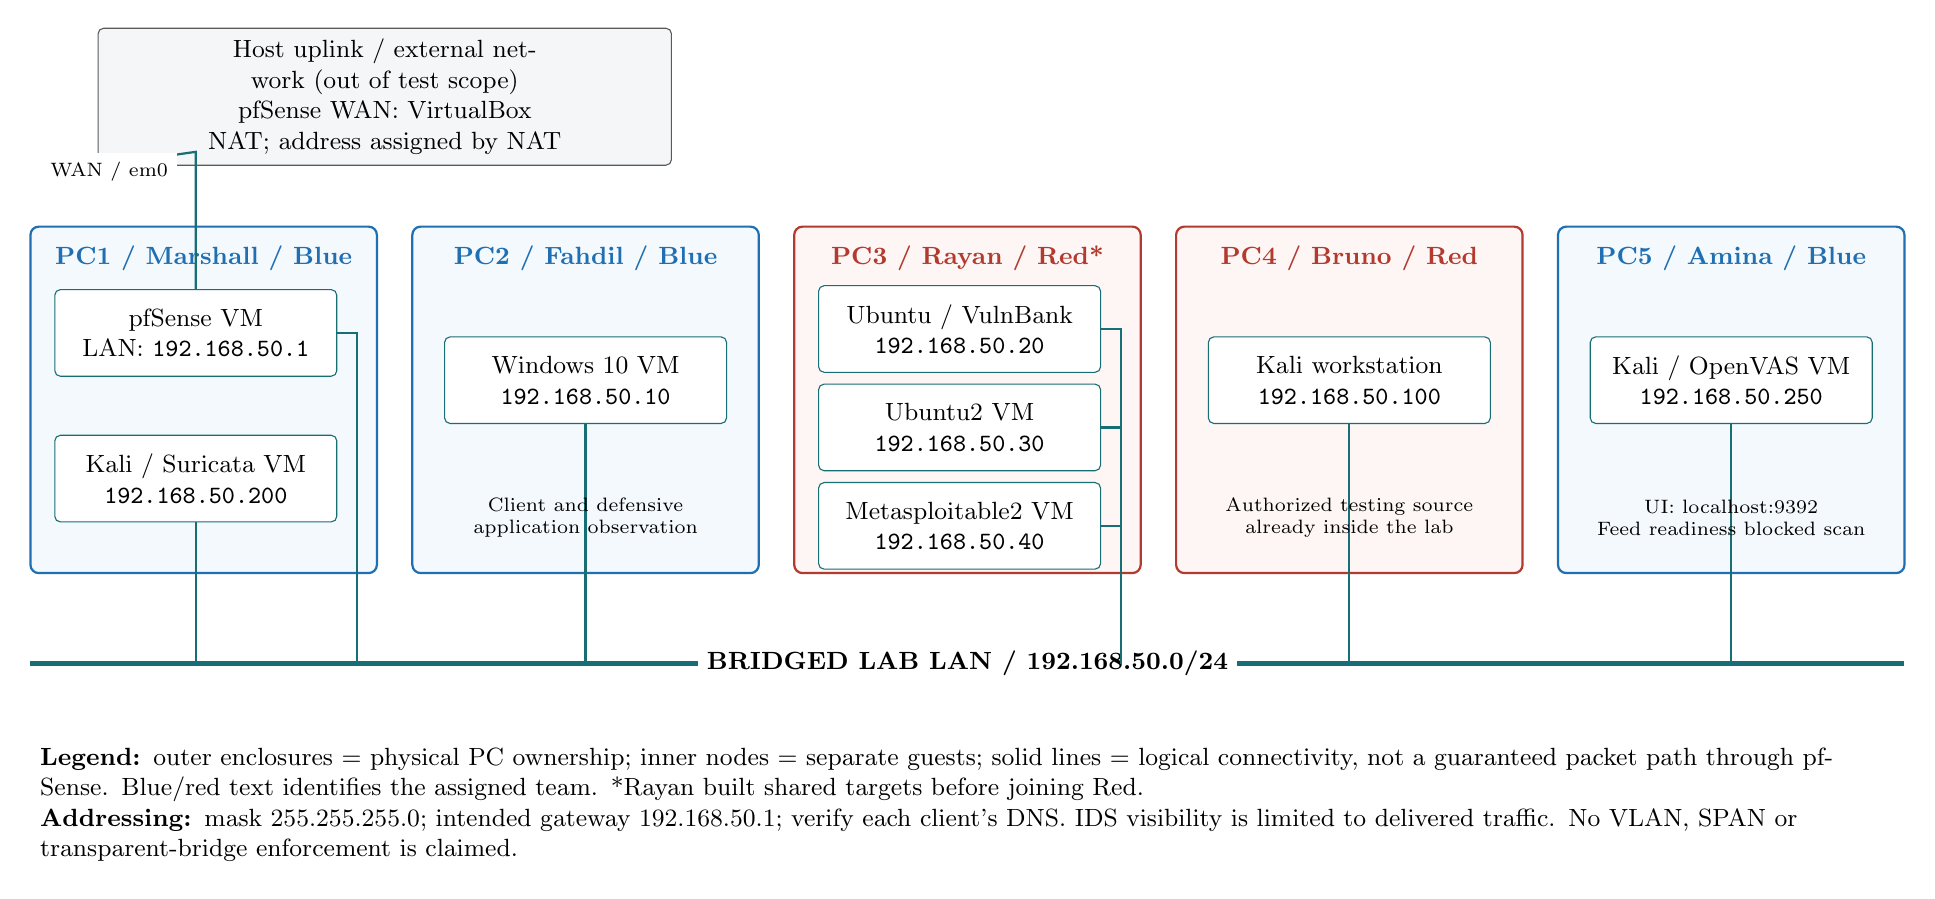
\begin{tikzpicture}[font=\small,
 guest/.style={draw=steel,fill=white,rounded corners=2pt,text width=3.3cm,minimum height=1.1cm,align=center,inner sep=4pt},
 host/.style={draw=blueteam,fill=blueteamlight!30,rounded corners=3pt,line width=0.8pt},
 wire/.style={draw=steel,line width=0.8pt},
 title/.style={font=\small\bfseries,align=center}]
\draw[host] (0,2) rectangle (4.4,6.4);
\draw[host] (4.85,2) rectangle (9.25,6.4);
\draw[host,draw=redteam,fill=redteamlight!30] (9.7,2) rectangle (14.1,6.4);
\draw[host,draw=redteam,fill=redteamlight!30] (14.55,2) rectangle (18.95,6.4);
\draw[host] (19.4,2) rectangle (23.8,6.4);
\node[title,text=blueteam] at (2.2,6.0) {PC1 / Marshall / Blue};
\node[title,text=blueteam] at (7.05,6.0) {PC2 / Fahdil / Blue};
\node[title,text=redteam] at (11.9,6.0) {PC3 / Rayan / Red*};
\node[title,text=redteam] at (16.75,6.0) {PC4 / Bruno / Red};
\node[title,text=blueteam] at (21.6,6.0) {PC5 / Amina / Blue};
\node[guest] (gw) at (2.1,5.05) {pfSense VM\\LAN: \texttt{192.168.50.1}};
\node[guest] (ids) at (2.1,3.2) {Kali / Suricata VM\\\texttt{192.168.50.200}};
\node[guest] (win) at (7.05,4.45) {Windows 10 VM\\\texttt{192.168.50.10}};
\node[guest] (app) at (11.8,5.1) {Ubuntu / VulnBank\\\texttt{192.168.50.20}};
\node[guest] (ubu) at (11.8,3.85) {Ubuntu2 VM\\\texttt{192.168.50.30}};
\node[guest] (meta) at (11.8,2.6) {Metasploitable2 VM\\\texttt{192.168.50.40}};
\node[guest] (atk) at (16.75,4.45) {Kali workstation\\\texttt{192.168.50.100}};
\node[guest] (gvm) at (21.6,4.45) {Kali / OpenVAS VM\\\texttt{192.168.50.250}};
\node[guest,draw=targetgrey,fill=lightgrey,text width=7cm] (up) at (4.5,8.05) {Host uplink / external network (out of test scope)\\pfSense WAN: VirtualBox NAT; address assigned by NAT};
\draw[wire,-{Latex}] (gw.north) -- (2.1,7.35) -- (up.south west);
\node[font=\scriptsize,fill=white] at (1.0,7.1) {WAN / em0};
\draw[wire,line width=2pt] (0,0.85) -- (23.8,0.85);
\node[fill=white,font=\small\bfseries] at (11.9,0.85) {BRIDGED LAB LAN / 192.168.50.0/24};
\draw[wire] (gw.east) -- (4.15,5.05) -- (4.15,0.85);
\draw[wire] (ids.south) -- (2.1,0.85);
\draw[wire] (win.south) -- (7.05,0.85);
\draw[wire] (app.east) -- (13.85,5.1) -- (13.85,0.85);
\draw[wire] (ubu.east) -- (13.85,3.85);
\draw[wire] (meta.east) -- (13.85,2.6);
\draw[wire] (atk.south) -- (16.75,0.85);
\draw[wire] (gvm.south) -- (21.6,0.85);
\node[font=\scriptsize,align=center,text width=3.6cm] at (7.05,2.7) {Client and defensive\\application observation};
\node[font=\scriptsize,align=center,text width=3.6cm] at (16.75,2.7) {Authorized testing source\\already inside the lab};
\node[font=\scriptsize,align=center,text width=3.6cm] at (21.6,2.7) {UI: localhost:9392\\Feed readiness blocked scan};
\node[align=left,text width=23cm,anchor=north west,font=\small] at (0,-0.1) {\textbf{Legend:} outer enclosures = physical PC ownership; inner nodes = separate guests; solid lines = logical connectivity, not a guaranteed packet path through pfSense. Blue/red text identifies the assigned team. *Rayan built shared targets before joining Red.\\\textbf{Addressing:} mask 255.255.255.0; intended gateway 192.168.50.1; verify each client's DNS. IDS visibility is limited to delivered traffic. No VLAN, SPAN or transparent-bridge enforcement is claimed.};
\end{tikzpicture}
\captionof{figure}{As-built ownership and logical connectivity. All eight lab addresses are shown in full; WAN connectivity and endpoint traffic are deliberately distinguished.}
\end{center}
\end{landscape}

\partheading{03 / BUILD JOURNEY}{Laboratory Setup and Readiness}
\label{sec:setup}
\subsection{Shared Preparation and the Host-Only Failure}
The team first created the virtual router and attempted to connect guests using host-only networking. That arrangement did not join guests across five separate physical PCs. A host-only network is normally local to one hypervisor; a cross-PC lab needs an explicitly shared network. The later screenshots show bridged adapters connected to the relevant physical Wi-Fi interfaces. The earlier failure is \textbf{team-reported}; the later adapter configuration is \textbf{observed}.

\begin{troublebox}[Difficulty Encountered - Host-Only Networking]
\textbf{Problem.} Our guests on different physical PCs could not communicate through the initial host-only arrangement. \textbf{Why.} Each host-only network was local to its own hypervisor; assigning matching IP prefixes did not join those separate networks. \textbf{Response.} We changed the lab-facing adapters to Bridged Adapter on the appropriate physical interfaces and retained the agreed static addresses. \textbf{Outcome.} The later bridged settings and eight-host discovery result corroborate shared-LAN connectivity (\ev{E004}, \ev{E005}, \ev{E030}). This overcame the reachability problem, not the separate need for isolation and verified monitoring coverage.
\end{troublebox}

The repeatable setup order is: install the hypervisor, create/import each guest, connect the correct adapter, install the guest OS, set addressing, validate the gateway and peer path, install or start the role-specific tools, then take a clean snapshot. Use trusted installation media and keep vulnerable images on an authorized lab-only physical network. NAT on pfSense's WAN is not, by itself, proof that a bridged LAN is isolated from every non-lab device. The actual snapshots and installer wizard sequence were not supplied; the steps below are a reconstruction supported by the configuration evidence, not screenshots of every installer screen.

\begin{tabularx}{\linewidth}{@{}L{2.9cm}X X@{}}
\toprule
\textbf{Machine} & \textbf{Build sequence} & \textbf{Readiness evidence}\\
\midrule
PC1 Marshall & Install pfSense in one guest and Kali in another; assign NAT WAN and bridged LAN to pfSense; configure gateway, then Suricata. & Adapter screenshots, configuration test, live logs and gateway capture.\\
PC2 Fahdil & Create Windows 10 guest from authorized media; bridge the lab NIC; apply the workstation's static address; verify application access. & Windows 10 browser session; shared early gateway setup captures.\\
PC3 Rayan & Create two Ubuntu guests; import Metasploitable2 as a separate guest; configure each address; start Apache/VulnBank. & Three adapter views, Netplan/interfaces files, Apache service and login page.\\
PC4 Bruno & Install Kali; configure the lab NIC and address; verify Nmap and Metasploit; create an evidence folder. & Tool banners, discovery output and source address on exploit session.\\
PC5 Amina & Install Kali/GVM; allocate disk and memory headroom; start services; complete feeds before target/task creation. & Service commands and working UI, but feed and target-creation gates failed.\\
\bottomrule
\end{tabularx}

\subsection{PC1: Marshall's Router and Separate Sensor}
\textbf{pfSense VM.} Create a FreeBSD-compatible virtual machine, attach the installer, install to its virtual disk and remove the installation medium after reboot. Map WAN and LAN using the actual NIC identifiers. The final PC1 captures show Adapter 1 set to NAT and Adapter 2 bridged to the host's MediaTek Wi-Fi interface with cable connected (\ev{E004}, \ev{E005}). Earlier shared setup captures in Fahdil's folder show pfSense 2.5.2; the containment shell shows 2.9.0. These are stages in the supplied record, not proof of two concurrent gateways.
\screenshot{E004}
\textbf{Next setup step.} Connect the second adapter to the shared lab segment, keeping it distinct from the NAT uplink.
\screenshot{E005}

In the console, assign WAN and LAN, choose \textbf{Set interface(s) IP address}, select LAN and enter \texttt{192.168.50.1/24}. Use a DHCP pool outside the static-address reservations only if DHCP is intentionally enabled; do not introduce a competing DHCP server on a shared uplink. Open \texttt{https://192.168.50.1} from an approved management client, review certificate identity, configure DNS forwarding/resolution as intended, and replace the initial administrator password. The later screenshot still displays the default-password warning, so password replacement is a required remediation, not a completed action in this report.
\textbf{Shared setup evidence.} The following console captures were supplied in Fahdil's folder. They illustrate interface assignment, LAN address entry and the resulting early console state; they are not attributed to the later PC1 session.
\screenshot{E015}
\textbf{Address entry.} Select the LAN interface and enter the intended gateway address.
\screenshot{E016}
\textbf{Console verification.} Check the displayed interface mapping and LAN address after configuration.
\screenshot{E012}

\textbf{Kali/Suricata VM.} Create a separate Linux guest on PC1, bridge its lab-facing interface and assign \texttt{192.168.50.200/24}. Determine the interface name from the guest rather than borrowing pfSense's \texttt{em1}. The observed Suricata configuration test is not proof that a long-running service has started; the later alert and statistics captures establish operation.
\textbf{Package preparation.} During setup, review the service-restart prompt generated by package maintenance before proceeding to the sensor checks.
\screenshot{E008}

\begin{cmdbox}[PC1 Kali - reproducible installation and configuration checks]
\begin{reportcode}
sudo apt update
sudo apt install suricata suricata-update jq tshark
ip -brief address
sudo nano /etc/suricata/suricata.yaml
sudo suricata-update
sudo suricata -T -c /etc/suricata/suricata.yaml -v
sudo systemctl enable --now suricata
sudo systemctl restart suricata
sudo systemctl status suricata --no-pager
\end{reportcode}
\end{cmdbox}
\textbf{Configuration decision.} Set the existing \texttt{vars: address-groups: HOME\_NET} entry to \texttt{[192.168.50.0/24]}, preserve valid YAML indentation, and set the capture interface in the configuration or service arguments actually used by the installed package. Inspect \texttt{systemctl cat suricata} if the service overrides the YAML. Enable the fast and EVE outputs needed for evidence. Do not add a second conflicting capture configuration or run two unintended Suricata instances.

\textbf{Meaning of the commands.} Package installation provides the sensor and review tools; \texttt{suricata-update} supplies the configured rule feed; \texttt{-T} tests configuration and rule loading; service status and fresh log timestamps verify ongoing operation. \ev{E009} displays Suricata 8.0.7, 53,098 rules loaded, zero failed and zero skipped in test mode. \ev{E007} supplies the stronger operational evidence: actual Nmap-labelled alerts. A replay or peer-generated test observed at the sensor is still needed to validate any additional capture path.
\screenshot{E009}

\subsection{PC2: Fahdil's Windows 10 Workstation}
Install Windows 10 in its own VirtualBox guest, finish the local lab-account setup, and bridge the lab NIC. In IPv4 properties set \texttt{192.168.50.10}, mask \texttt{255.255.255.0}, gateway \texttt{192.168.50.1}, and the verified lab DNS resolver. Install Guest Additions if required for display usability; shared clipboard/folders should be disabled during hostile testing unless explicitly needed.
\textbf{Preparation inventory.} Fahdil's early VirtualBox view establishes which local guests were present. The selected settings describe the early pfSense guest, not the Windows guest's hardware.
\screenshot{E013}
\textbf{Shared gateway preparation.} The following bridged-adapter view belongs to that early pfSense configuration; the final PC1 arrangement was shown in the preceding subsection.
\screenshot{E014}

\begin{cmdbox}[PC2 Windows PowerShell - identity and connectivity checks]
\begin{reportcode}
hostname
whoami
Get-Date -Format o
ipconfig /all
ping -n 4 192.168.50.1
Test-NetConnection 192.168.50.20 -Port 80
Get-NetFirewallProfile | Select-Object Name, Enabled
net accounts
\end{reportcode}
\end{cmdbox}
These are \textbf{rebuild/verification instructions}, not claimed historical transcript lines. They establish identity, prefix, gateway, DNS, service reachability and the local firewall/password-policy baseline. \texttt{::} comments belong to Command Prompt, not PowerShell; PowerShell comments use \texttt{\#}. Preserve Windows Firewall while diagnosing any failed ping and use a narrowly scoped test rule instead of disabling all protection.

\ev{E017}--\ev{E019} show Fahdil accessing VulnBank from a running Windows 10 guest and viewing an administrative application session. An earlier inventory has WINDOWS10 powered off, but that does not describe the whole test day. No Windows Security event export, applied password-policy change or host-firewall block was supplied, so those defensive controls remain verification items. In a production analogue, use a supported Windows release or documented extended support rather than assuming Windows 10 is currently patched.
\screenshot{E017}

\subsection{PC3: Rayan's Application and Target Guests}
Rayan first prepared the shared infrastructure, then joined the Red Team. The evidence shows separate guests named \texttt{ubuntu\_server}, \texttt{Ubuntu2} and \texttt{METASPLOITABLE 2}; it does not show a nested-hypervisor or Docker/macvlan deployment. Their bridged NIC settings appear in \ev{E025}--\ev{E027}.
\textbf{Connect the application guest.} Verify its bridged adapter and review the secondary NAT connection before testing.
\screenshot{E027}
\textbf{Connect Ubuntu2.} Use the shared lab interface and a distinct guest adapter identity.
\screenshot{E026}
\textbf{Connect Metasploitable2.} Review both adapters so the vulnerable guest has no unintended route outside the authorized segment.
\screenshot{E025}

\textbf{Ubuntu addressing.} The actual Netplan file is \texttt{/etc/netplan/50-cloud-init.yaml}, and the visible interface is \texttt{enp0s3}. The server screenshot shows its \texttt{192.168.50.20/24} address but not a route/DNS entry; Ubuntu2 explicitly shows \texttt{192.168.50.30/24}, gateway \texttt{192.168.50.1} and DNS \texttt{192.168.50.1}. Do not infer omitted fields from the other guest. For a repeatable rebuild, inspect existing cloud-init ownership and other Netplan files before editing; avoid two definitions competing for the same interface.
\screenshot{E022}

\begin{cmdbox}[Ubuntu2 - configuration transcribed from E023]
\begin{reportcode}
network:
  version: 2
  ethernets:
    enp0s3:
      dhcp4: no
      addresses:
        - 192.168.50.30/24
      routes:
        - to: default
          via: 192.168.50.1
      nameservers:
        addresses: [192.168.50.1]
\end{reportcode}
\end{cmdbox}
      \screenshot{E023}
\begin{cmdbox}[Ubuntu - validation steps for a controlled rebuild]
\begin{reportcode}
ip -brief address
sudo netplan generate
sudo netplan try
ip route
resolvectl status
ping -c 4 192.168.50.1
\end{reportcode}
\end{cmdbox}
\texttt{generate} checks configuration generation; \texttt{try} provides timed rollback if connectivity is lost. Review/confirm from the VM console. For the server, use its assigned \texttt{192.168.50.20/24}; add route/resolver values only after verifying the intended network. Do not rerun address-changing commands over the only remote administrative connection without recovery access.

\textbf{Application service.} \ev{E029} shows the Apache sites \texttt{000-default.conf} and \texttt{vul-bank.conf}, followed by an active Apache service. \ev{E020} shows a local Windows hosts-file entry mapping \texttt{vul-bank.duckdns.org} to \texttt{192.168.50.20}; this is lab name resolution, not evidence of a DNS-spoofing attack. The initial \texttt{nodpath} typo is followed by \texttt{notepad hosts}. The screenshots do not preserve the application checkout, dependency install or Node service definition; no invented repository or installation command is supplied.
\screenshot{E020}
\begin{troublebox}[Difficulty Encountered - Hosts-File Command Typo]
\textbf{Problem.} The first attempt to open the hosts file failed with an unrecognized-command message. \textbf{Why.} We entered \texttt{nodpath}, which was not the intended editor command. \textbf{Response.} The capture shows the corrected \texttt{notepad hosts} command and the lab mapping to \texttt{192.168.50.20}. \textbf{Outcome.} The file could be opened and the later browser view reached VulnBank by its lab hostname. This was a local command-entry problem, not an attack on DNS.
\end{troublebox}
\textbf{Check application reachability.} After the local name mapping, open the lab hostname and confirm that the intended demo application is returned.
\screenshot{E028}

\begin{cmdbox}[PC3 Ubuntu - observed service check and recommended verification]
\begin{reportcode}
ls /etc/apache2/sites-enabled/*.conf
systemctl status apache2

# Follow-up checks; results were not supplied for these commands.
sudo apache2ctl configtest
sudo ss -lntp
curl -I http://192.168.50.20
curl -I http://192.168.50.20:3000
\end{reportcode}
\end{cmdbox}
The service status establishes that Apache is running, not that VulnBank is secure. Later remote headers identify Apache 2.4.58 and Express on ports 80/3000. Exposing the application directly on 3000 is an additional route to assess; identical page lengths do not prove identical access controls.
\screenshot{E029}

\textbf{Metasploitable2.} Import the supplied vulnerable image into an isolated lab guest, verify its architecture, and keep it separate from production credentials. The legacy interfaces file in \ev{E024} uses \texttt{eth0} and includes loopback configuration. Preserve loopback and replace only the intended NIC stanza when reconstructing it.
\begin{cmdbox}[Metasploitable2 - observed static interface stanza]
\begin{reportcode}
auto eth0
iface eth0 inet static
    address 192.168.50.40
    netmask 255.255.255.0
    gateway 192.168.50.1
\end{reportcode}
\end{cmdbox}
  \screenshot{E024}
The corresponding legacy restart is \texttt{sudo /etc/init.d/networking restart}; verify with \texttt{ifconfig eth0} and a peer connection. Netplan and modern systemd commands do not apply automatically to this old guest. The supplied VM inventory also shows a NAT adapter at one stage; review and remove unintended secondary uplinks before retesting because they can bypass the intended lab boundary. \ev{E021} shows failed console logins later in the exercise, consistent with access disruption but not sufficient on its own to identify the cause.

\subsection{PC4: Bruno's Kali Attack Workstation}
Install Kali from trusted media, allocate enough host resources for the tools without starving the other guests, bridge the lab NIC, and apply \texttt{192.168.50.100/24}. A typical Kali desktop uses NetworkManager; it should not be assumed to have Ubuntu's Netplan layout. Use the existing NetworkManager connection in the GUI to set manual IPv4, gateway and DNS, then reconnect from the local VM console. Exact VM disk/RAM values for PC4 were not captured and are not asserted as measured facts.
\begin{cmdbox}[PC4 Kali - readiness before the recorded reconnaissance]
\begin{reportcode}
nmcli connection show --active
ip -brief address
ip route get 192.168.50.40
ping -c 4 192.168.50.1
nmap --version
msfconsole --version
hydra -h
whatweb --version
mkdir -p ~/CYS4151/evidence
\end{reportcode}
\end{cmdbox}
These checks identify the actual NIC and route, verify the gateway and tool availability, and prepare a local evidence directory. Do not perform blanket upgrades midway through an assessment without a snapshot and a recorded version change. The execution screenshots identify Nmap 7.95, Hydra 9.5 and a Metasploit 6.4.84-dev banner. The corrupt Zsh history warning in \ev{E033} is a tooling issue, not proof the target resisted testing.

\subsection{PC5: Amina's Kali/OpenVAS Scanner}
Amina's dedicated PDF reports an initial RAM increase from 2,000 MB to 4,000 MB to clear an installation problem, followed by a disk increase from 30 GB to 80 GB, 8,000 MB RAM and two processors for the feed attempts. The earlier team account emphasized disk shortage. Both are recorded as \textbf{reported resource interventions}; neither explains all later errors. The screenshots of video-memory settings are not proof that VRAM caused GVM's feed failure.
\begin{troublebox}[Difficulty Encountered - Scanner VM Resources]
\textbf{Problem.} We encountered resource problems while preparing OpenVAS. The team reported insufficient disk space, and Amina also documented an initial installation error addressed by increasing system RAM. \textbf{Response.} Her report records disk expansion from 30 GB to 80 GB and later allocation of 8,000 MB RAM and two processors. \textbf{Outcome.} Services and the local web interface became available, but the subsequent feed/import problems remained. These changes addressed reported setup constraints; they did not prove that all additional disk space was usable or that scanning was ready. Video memory was not the same resource as RAM or disk.
\end{troublebox}
\textbf{Prepare evidence capture.} Amina first adjusted the host terminal's input and selection properties. These are recording-environment settings, not scanner results.
\screenshot{E054}
\textbf{Confirm terminal settings.} The second supplied view documents the same preparation at a closer scale; it is reproduced in full as received.
\screenshot{E055}
\textbf{Review VM settings.} The VirtualBox warning must be interpreted from its actual details before assigning a cause to it.
\screenshot{E071}
\textbf{Distinguish resource types.} The next settings screen concerns display memory, which must not be confused with system RAM or disk capacity.
\screenshot{E072}
\begin{troublebox}[Difficulty Encountered - VirtualBox Settings Warning]
\textbf{Problem.} VirtualBox displayed \texttt{Invalid settings detected} while we reviewed the VM settings. \textbf{Why.} The warning details were not expanded in the supplied captures, so the exact incompatible setting is unknown. \textbf{Response and outcome.} We recorded the settings review, but no confirmed correction of this warning is shown. It must not be presented as proof that increasing video memory fixed OpenVAS.
\end{troublebox}

\begin{cmdbox}[PC5 Kali - observed service and feed commands]
\begin{reportcode}
sudo systemctl start ospd-openvas
sudo systemctl start notus-scanner
sudo systemctl start gsad
sudo tail -f /var/log/gvm/gvmd.log
sudo greenbone-feed-sync --type all
watch -n 15 sudo du -sh /var/lib/gvm/scap-data/
\end{reportcode}
\end{cmdbox}
\textbf{Service startup evidence.} The first three commands in the block are visible in the following capture. The later log and synchronization operations appear with their matching screenshots in the Task 5 scanning phase.
\screenshot{E048}
\textbf{Identity-bearing startup record.} A second, separately supplied capture preserves Amina's name alongside the startup commands.
\screenshot{E056}
Service starts are visible in \ev{E048}/\ev{E056}; the log path and sync command are visible in \ev{E073}/\ev{E074}. The screenshots show GSA at \texttt{127.0.0.1:9392}. Configure the lab-facing NIC as \texttt{192.168.50.250/24} and verify the route before scanning; \ev{E050} corroborates that address in ICMP traffic. A second NAT address is visible during feed troubleshooting, so direct uplinks should be reviewed before any containment test.
\textbf{Open the local web interface.} An initial administrative login failed. This is part of bringing the scanner up, not an attack against a target host.
\screenshot{E057}
\begin{troublebox}[Difficulty Encountered - GSA Login Rejected]
\textbf{Problem.} The local scanner portal returned \texttt{Invalid password or username}. \textbf{Why.} The submitted credentials were not accepted; the image does not distinguish a wrong username from a wrong password. \textbf{Response.} We retried access before proceeding to the task list. \textbf{Outcome.} The later authenticated GSA views show that portal access resumed, but the exact credential correction or reset was not recorded. The next obstacle was feed readiness, not portal reachability.
\end{troublebox}

\textbf{Readiness gate.} An accessible GSA login is not a ready scanner. The feed owner, imported port lists, scan configurations, scanner connection and selected feed versions must be usable before a target/task can be created. Amina's target list attempt included additional lab hosts in some views; no complete successful target definition or scan launch is demonstrated. The final outcome appears in Section~\ref{phase:assessment}.

\subsection{Problems Encountered and Lessons Applied}
\begin{tabularx}{\linewidth}{@{}L{3.1cm}X X@{}}
\toprule
\textbf{Problem} & \textbf{Response and evidence} & \textbf{What remains important}\\
\midrule
Host-only across physical PCs & Team reported failed inter-PC reachability; later settings show bridged adapters. & Bridging fixes reachability, not security isolation or guaranteed IDS visibility.\\
Resource pressure on PC5 & Disk/RAM increases reported; service and feed troubleshooting captured. & Check guest filesystem capacity as well as virtual disk size; do not assume feed import is fixed.\\
Feed owner / port list absent & Repeated target creation, log inspection and full-feed synchronization. & No completed scan; preserve error evidence and rerun after readiness checks.\\
Copy-pasted command flags & Earlier PDFs produced typographic hyphens; corrected PDF text mapping is retained here. & Verify extracted commands contain ASCII hyphen-minus, not just that glyphs look correct.\\
Malformed EVE input & Team encountered a repeated JSON parse error; fast.log remained readable. & Preserve the bad line and investigate its origin. A partial write is only one hypothesis.\\
Mixed local clocks & Guest EDT and other local/UTC displays appear together. & Preserve offsets and correlate carefully; do not invent response-time statistics.\\
\bottomrule
\end{tabularx}

\partheading{04 / EXERCISE SEQUENCE}{From Reconnaissance to Demonstrated Impact}
\label{sec:red}
\subsection{Strategy and Initial Position}
\textbf{Red Team voice: Bruno (PC4), with Rayan (PC3) after infrastructure setup.} We began on Kali at \texttt{192.168.50.100}, already connected to the authorized lab. We therefore did not need to break through an Internet perimeter. Our first question was which systems were reachable and what they exposed. We wanted each test to answer that question more precisely before we attempted controlled access.

Our strategy was to narrow the attack surface in stages. We first discovered live addresses, then identified their services, then checked the access policies of the services that looked most relevant. Those results led us to two different targets: Metasploitable2 at \texttt{192.168.50.40} for the server-side path, and VulnBank at \texttt{192.168.50.20} for the application path. We did not assume that access to one meant access to the other.

For each path, we followed the same reasoning: establish the service, choose a matching test, inspect the actual response, and verify the resulting access before describing its impact. When an attempt failed or a tool produced conflicting output, we retained that result and explained the next decision. The narrative below follows the exercise phases; it does not turn an expected outcome from the setup guide into a claim that we achieved it.

\begin{center}
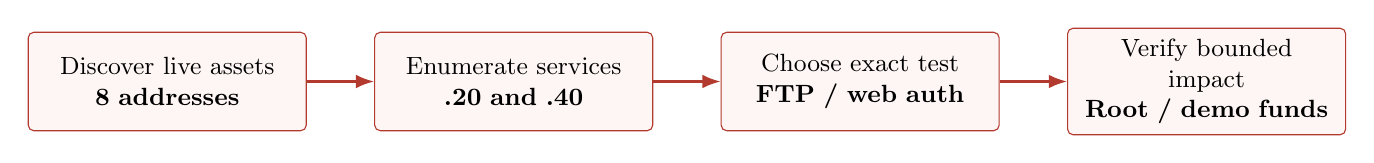
\begin{tikzpicture}[font=\small,stage/.style={draw=redteam,fill=redteamlight!30,rounded corners=2pt,text width=3.25cm,minimum height=1.25cm,align=center,inner sep=4pt}]
\node[stage] (discover) at (0,0) {Discover live assets\\\textbf{8 addresses}};
\node[stage] (enumerate) at (4.4,0) {Enumerate services\\\textbf{.20 and .40}};
\node[stage] (select) at (8.8,0) {Choose exact test\\\textbf{FTP / web auth}};
\node[stage] (verify) at (13.2,0) {Verify bounded impact\\\textbf{Root / demo funds}};
\draw[-{Latex},redteam,thick] (discover) -- (enumerate);
\draw[-{Latex},redteam,thick] (enumerate) -- (select);
\draw[-{Latex},redteam,thick] (select) -- (verify);
\end{tikzpicture}
\captionof{figure}{Red Team decision sequence. Each transition requires an observed result rather than assuming the preparatory guide succeeded.}
\end{center}

\subsection{Reconnaissance: Establish the Asset Map (Task 2)}
\label{phase:recon}
Before selecting an exploit, we needed an inventory of the systems actually online. We chose \texttt{nmap -sn} because it performs host discovery without following it with a port scan. This gave us a manageable starting list and avoided running service tests against addresses that had not yet responded.
\begin{cmdbox}[Recorded on PC4 Kali - discovery]
\begin{reportcode}
nmap -sn 192.168.50.0/24
\end{reportcode}
\end{cmdbox}
The sweep reported eight live addresses, including our own Kali machine. We used those responses to build the asset map for the next step. On a directly connected Ethernet-style subnet, a privileged Nmap run normally uses ARP discovery; probe behaviour depends on privilege and path. We treated this as active discovery, not invisible reconnaissance, and did not assume it would produce a TCP port-scan alert.

\reportfigure{E030}{Complete discovery screenshot, \ev{E030}.}{Eight hosts are reported up in 8.35 seconds, including the attacker's own address. The no-DNS-server warning does not invalidate discovery by numeric IP. MAC vendor labels repeat across several bridged guests and should not be treated as authoritative operating-system evidence.}

\begin{troublebox}[Difficulty Encountered - Nmap DNS Warning]
\textbf{Problem.} Nmap warned that it could not determine DNS servers and disabled reverse-DNS resolution. \textbf{Why.} Resolver information was unavailable to that scan; the screenshot does not establish the underlying configuration cause. \textbf{Response.} We continued with the authorized numeric IP addresses rather than relying on hostnames. \textbf{Outcome.} Discovery still returned eight live addresses, allowing service enumeration to proceed. This was a working bypass of the naming dependency, not evidence that DNS itself was repaired.
\end{troublebox}

Having established who was online, our next question was what each host was running. We kept the gateway, workstation, sensor and scanner in the inventory, then used service identification to decide where a controlled exploitation test would be most useful. That next pass, rather than the discovery result alone, led us to concentrate on \texttt{192.168.50.20} and \texttt{192.168.50.40}.

\subsection{Scanning and Service Enumeration (Task 3)}
\label{phase:scanning}
We moved from addresses to services using the per-host \texttt{-A} pass recorded in our Red Team report. We chose it to collect service versions, default-script results, OS hints and traceroute information together, and used \texttt{-oN} to retain normal text output. Some parts of that scan require appropriate privileges and responsive ports, so we treated guessed OS labels as hints rather than confirmed identities. Not every per-host result was preserved; the following captures show the results available for our target selection.
\screenshot{E031}
The application host exposed VulnBank on ports 80 and 3000, which gave us a web-assessment path. Metasploitable exposed a much broader collection of legacy services, which gave us a separate server-side path. We inspected that second result before deciding which service to test first.
\screenshot{E032}

\subsubsection{Scan the Selected Hosts Across the TCP Port Range}
The initial service results were useful, but we still needed to check for listeners outside the default port selection. We therefore ran a full TCP port scan against the two chosen targets. Keeping the target list explicit also kept this deeper test within the systems we had selected for the exercise.
\begin{cmdbox}[Recorded PC4 command - full TCP service scan]
\begin{reportcode}
nmap -sV -sC -p- 192.168.50.20 192.168.50.40 -oN full_scan.txt
\end{reportcode}
\end{cmdbox}
We used \texttt{-sV} for service versions, \texttt{-sC} for default NSE checks, \texttt{-p-} for TCP ports 1--65535, and \texttt{-oN} to save the result. On the application host, the displayed output again identified the three relevant listeners: SSH, HTTP and Express. That helped us move on to web fingerprinting instead of continuing to search blindly for another TCP service. The scan did not cover all UDP services or every application route, so it was not a complete security assessment by itself.
\screenshot{E033}
\begin{troublebox}[Difficulty Encountered - Corrupt Shell History]
\textbf{Problem.} Kali displayed a corrupt Zsh history-file warning. \textbf{Why.} The shell could not read its history normally; the original cause of the file damage was not established. \textbf{Response.} We continued issuing the required commands directly and retained their displayed results rather than depending on history alone. \textbf{Outcome.} The Nmap scan still ran. No repair of the history file is evidenced, and the warning was not a target-side security control.
\end{troublebox}

\begin{tabularx}{\linewidth}{@{}L{3.1cm}L{3.0cm}X@{}}
\toprule
\textbf{Target} & \textbf{Visible service} & \textbf{Decision supported}\\
\midrule
192.168.50.20 & 22/TCP, OpenSSH 9.6p1 & Administrative service; no successful SSH exploitation of this host is shown.\\
192.168.50.20 & 80/TCP, Apache 2.4.58 & Inspect VulnBank and its login/administrative functions.\\
192.168.50.20 & 3000/TCP, Express & Compare the direct application listener with the HTTP front end.\\
192.168.50.30 & 22/TCP in initial view & Retain as Ubuntu2 infrastructure; the visible evidence does not justify a DVWA-specific attack.\\
192.168.50.40 & 21/TCP, vsftpd 2.3.4 & Validate anonymous FTP and investigate the matching backdoor module.\\
192.168.50.40 & SMB, old SSH and other services & Enumerate access policy; treat remaining services as leads pending individual validation.\\
\bottomrule
\end{tabularx}

\subsubsection{Fingerprint the Web Listeners}
With two web listeners on \texttt{192.168.50.20}, we wanted to know whether they exposed the same application and which technologies answered on each port. We used WhatWeb to identify visible web technologies and \texttt{curl -I} to inspect response headers without retrieving a full page body. This helped us choose application-specific tests rather than applying the DVWA instructions to a different application.
\begin{cmdbox}[Recorded PC4 commands - web technology and HTTP headers]
\begin{reportcode}
whatweb 192.168.50.20
whatweb 192.168.50.20:3000
curl -I http://192.168.50.20
curl -I http://192.168.50.20:3000
\end{reportcode}
\end{cmdbox}
\reportfigure{E034}{Complete HTTP fingerprinting and header screenshot, \ev{E034}.}{Both HTTP listeners return 200 responses and a 2778-byte page; Apache and Express headers identify the stack. The displayed HTTPS connection refusal supports the cleartext-service concern. Matching lengths do not prove identical authorization or that traffic on port 3000 passes through Apache.}
These responses confirmed VulnBank as our web target and gave us a separate transport-security concern to record. We then returned to Metasploitable's service list: before choosing an exploit, we wanted to establish whether its file-transfer and file-sharing services also allowed unintended access.

\subsubsection{Validate Anonymous Service Access}
Open ports alone did not tell us whether authentication was enforced. We chose \texttt{smb-enum-shares} to inspect the exposed SMB shares and \texttt{ftp-anon} to test anonymous FTP authentication. Each script answered a specific question raised by the preceding service scan.
\begin{cmdbox}[Recorded PC4 commands - access-policy checks]
\begin{reportcode}
nmap --script=smb-enum-shares -p445 192.168.50.40
nmap --script=ftp-anon -p21 192.168.50.40
\end{reportcode}
\end{cmdbox}
The SMB output classified the \texttt{tmp} share as anonymous \texttt{READ/WRITE}; the FTP check returned \texttt{230}, indicating that anonymous authentication was accepted. We now had concrete access-policy findings rather than just a list of open ports. We retained both results for remediation, while avoiding a claim of file theft because no such operation was demonstrated.
\screenshot{E035}
\textbf{Read the continuation and FTP result.} The second capture completes the share-access output and records the separate anonymous FTP check.
\screenshot{E036}

We chose the FTP path for our controlled initial-access test because the exact vsftpd banner gave us a specific backdoor hypothesis to investigate. The anonymous-access checks strengthened our assessment of the host's permissive configuration, but they did not themselves prove that the backdoor was present. Those are different weaknesses: disabling anonymous login would not repair a backdoored binary. We also noted \texttt{distccd} as a backup lead in our report, but did not demonstrate a separate exploit against it.

\subsection{Threat Modelling and Test Selection (Task 4)}
\label{phase:threat}
At this point, we translated the service observations into a test plan: what asset could be affected, what access an attacker might gain, and what bounded test could confirm or reject the hypothesis. This connects our reconnaissance to the later exploitation choices. The table is analysis based on the preceding evidence, not a separate captured threat-modelling session; the final findings chapter develops the ratings after considering the test results.
\begin{tabularx}{\linewidth}{@{}L{3.2cm}X X@{}}
\toprule
\textbf{Asset / lead} & \textbf{Potential consequence} & \textbf{Next justified test}\\
\midrule
Metasploitable FTP banner & Possible remote execution if the backdoor is present & Review the exact module, then verify target identity and resulting privileges in a controlled test.\\
Anonymous SMB/FTP access & Unintended file access or modification & Preserve access-policy evidence; do not claim file theft without a separate test.\\
VulnBank HTTP and login & Credential exposure or misuse of privileged application functions & Examine the real login request, test the selected input and verify any candidate credentials independently.\\
Firewall and monitoring & Unnoticed activity or incomplete containment & Start observation before testing; identify the source and later verify the exact path affected by a block.\\
\bottomrule
\end{tabularx}

\subsection{Vulnerability Scanning: Amina's OpenVAS Attempt (Task 5)}
\label{phase:assessment}
\textbf{Blue Team voice: Amina on PC5.} We wanted an independent vulnerability assessment to complement the Red Team's manual enumeration. OpenVAS was intended to give us broader coverage, after which we could compare its findings with targeted manual checks and prioritize remediation. We therefore needed a working scanner, usable feeds and a valid target before trusting any results.

Our preparation ran alongside Red Team work; this section appears before initial access to follow the exercise phases. It did not produce a completed scan that enabled the later exploit. Instead, we encountered a sequence of readiness problems and recorded the outcome as \textbf{Incomplete - assessment blocked}. The Red Team proceeded from its manual service evidence, not an OpenVAS report that did not exist.
\subsubsection{Open the Task List and Check Readiness}
After reaching GSA, we checked the task list rather than immediately assuming the scanner was ready. It showed no tasks and explicitly said that scans were unavailable while the feeds synchronized. This told us to investigate readiness before interpreting the absence of results as anything about the target network.
\screenshot{E058}
We revisited the task list, but still had no scan task. A later frame showed an inactivity warning instead of the feed banner; that was not enough to conclude that import had finished. We therefore moved to the feed-status page to check the individual components directly.
\screenshot{E059}

\reportfigure{E060}{OpenVAS feed-status evidence: NVT Current while SCAP is still importing (\ev{E060}).}{Different feeds have different functions. GVMD Data supplies port lists and scan configurations; SCAP supplies vulnerability/product metadata. A SCAP progress message alone is not the direct explanation of an absent default port list. The accompanying feed-owner and GVMD-data errors establish the broader readiness gap.}

\subsubsection{Attempt Target Creation and Preserve Each Error}
We entered the intended lab addresses in a target named \texttt{CYS4151-Targets}. Creating this object was necessary before a scan task could refer to it. Our first dialog records the intended configuration, but not a successful save, so we retained the later error messages to explain why we could not progress.
\screenshot{E049}
We tried saving the target again and kept this second configuration view so the attempted scope remained visible alongside the failure.
\screenshot{E061}
The next message said the feed owner was not set. This pointed us back to the scanner's own prerequisites rather than to a security weakness on the selected hosts.
\screenshot{E062}
A subsequent attempt reported that the default port list was unavailable. We needed that list to define the intended scan coverage, so the error stopped us before launch and justified inspecting the manager's imported data.
\screenshot{E063}
\textbf{Preserve the repeated failure.} The second full-dialogue view corroborates that the error persisted, rather than adding another independent finding.
\screenshot{E064}

\reportfigure{E065}{The default-port-list error that blocked target creation (\ev{E065}).}{The failure occurs before a scan task is launched. It cannot support a finding that the selected target hosts are secure or vulnerable, nor a scanner-derived severity chart.}
\begin{troublebox}[Difficulty Encountered - Missing Feed Owner and Port List]
\textbf{Problem.} We could not save the target because GVM reported an unset feed owner and an unavailable default port list. \textbf{Why.} Required scanner data/configuration was not ready; GVMD Data supplies the default port lists and scan configurations. The evidence does not isolate the underlying reason that those objects were missing. \textbf{Response.} We checked Feed Status, inspected manager logs, retried target creation and attempted synchronization. \textbf{Outcome.} The task remained blocked. No completed scan or CVSS export was produced, so this difficulty is recorded as unresolved rather than as an obstacle we successfully overcame.
\end{troublebox}

\subsubsection{Inspect Service Logs and Revisit Feed Status}
The interface told us what was missing, but not enough about why. We therefore inspected the manager logs to see which data GVM was failing to read. The missing \texttt{feed.xml} messages gave us a more precise troubleshooting lead than repeatedly changing the target name.
\screenshot{E051}
\textbf{Corroborate the warning with identity context.} The next supplied view preserves the same class of error with Amina's overlay.
\screenshot{E070}
We also used \texttt{sudo tail -f /var/log/gvm/gvmd.log} to follow new manager messages as they appeared. It reported that the scanner had not yet supplied a feed version and was still starting. That helped us distinguish an accessible web interface from an assessment engine that was actually ready.
\screenshot{E073}
We returned to Feed Status to compare those messages with the interface. NVT was Current while SCAP remained in progress, so we could not use the status of one component as proof that the whole scanner was ready.
\screenshot{E066}
\textbf{Later status checkpoint.} SCAP remains in progress in this additional supplied view.
\screenshot{E069}

\subsubsection{Synchronize and Measure Progress Without Assuming Completion}
We next ran \texttt{sudo greenbone-feed-sync --type all} to request the configured feeds together. The output showed a lock acquisition and the start of Notus/NASL downloads. This told us the synchronization process had begun, so our next step was to monitor progress and later recheck imported objects; it did not justify claiming a successful scan.
\screenshot{E074}
We looked at the traffic view to understand the active download path. It showed a NAT-side address communicating with the feed service. The external troubleshooting advice visible beside it was reference material, not proof that every suggested command had been executed.
\screenshot{E075}
We used \texttt{watch -n 15 sudo du -sh /var/lib/gvm/scap-data/} because repeated directory-size readings could show whether local feed data was growing. The first timed checkpoint showed 998M. This measured usage, not free disk space or database-import completion.
\screenshot{E078}
Thirty seconds later, the monitor showed 1002M. That gave us evidence of local growth and a reason to continue checking, but no completed target or task was yet demonstrated.
\screenshot{E079}
\textbf{Retain the separately supplied view of this checkpoint.} It supports the same usage reading, not another completed import.
\screenshot{E052}
The later reading reached 1.1G. We still needed GVM to expose the required data objects and accept a target; a larger directory alone could not answer that question.
\screenshot{E053}
\textbf{Preserve the final identity-bearing checkpoint.} The later capture and Amina's dedicated PDF both belong to the incomplete attempt.
\screenshot{E080}
\textbf{Check whether scans are available.} The supplied notification still describes synchronization as blocking scan availability.
\screenshot{E076}
We also retried with the target name \texttt{vul}, but the missing-port-list error persisted. This confirmed that changing the target name had not removed the readiness obstacle. We ended the documented attempt without a launched scan and carried the blocker into the remediation plan.
\screenshot{E077}
\begin{troublebox}[Difficulty Encountered - Synchronization Never Reached Readiness]
\textbf{Problem.} Feed files grew, but the scanner still could not create the intended target. \textbf{Why.} Downloaded directory content and imported, usable scan objects are different stages; the exact cause of the remaining import failure was not established. \textbf{Response.} Amina's report records five attempts, resource increases, log inspection and progress monitoring. \textbf{Outcome.} The final record remained incomplete. The next required work is a controlled feed-owner/import investigation and readiness retest, not another claimed successful vulnerability scan.
\end{troublebox}

\begin{tabularx}{\linewidth}{@{}L{3.4cm}X X@{}}
\toprule
\textbf{Checkpoint} & \textbf{Observed evidence} & \textbf{Why the next step followed}\\
\midrule
Service start & ospd-openvas, notus-scanner and gsad invoked & Open the local GSA interface and inspect readiness.\\
Feed review & NVT Current; SCAP Update in progress & Inspect import and metadata state rather than assuming the UI implies readiness.\\
Target creation & Feed-owner / default Port List errors & Examine gvmd logs and required data objects.\\
Log investigation & Missing feed.xml; scanner feed version unavailable & Attempt controlled synchronization and monitor import progress.\\
Full feed sync & Lock acquired; Notus/NASL downloads start & Allow completion, then verify actual imported port lists and scan configs.\\
Last recorded state & 998M, 1002M, then 1.1G SCAP directory; no scan & Record an incomplete task and schedule a separate retest after readiness.\\
\bottomrule
\end{tabularx}

\textbf{Resource history and uncertainty.} Amina reports five attempts, including a final run of roughly an hour, and the increases to disk/RAM/CPU described in the setup chapter. The snapshots measure directory usage, not free disk capacity, and do not prove that all enlarged disk space became usable inside the guest. The deeper cause of incomplete download/import was not isolated; rate limiting, locks, feed ownership, connectivity, version compatibility and filesystem capacity are investigation leads, not established causes.

\begin{cmdbox}[Recommended PC5 readiness diagnostics before a new scan attempt]
\begin{reportcode}
df -h
df -i
lsblk -f
free -h
sudo gvm-check-setup
sudo systemctl status gvmd ospd-openvas gsad --no-pager
sudo journalctl -u gvmd -u ospd-openvas -n 100 --no-pager
greenbone-feed-sync --help
\end{reportcode}
\end{cmdbox}
For a follow-up, we would use these diagnostics to separate remaining resource constraints from service and feed-import problems: \texttt{df} checks filesystem capacity and inodes, \texttt{lsblk} checks the disk layout, and \texttt{free} checks RAM. The GVM setup and service-log checks would then identify the next actionable failure. This is our proposed next investigation, not a set of completed historical fixes. We would follow the installed version's guidance, avoid overlapping syncs or deleting an active lock, and require a valid feed owner, port list, scan configuration and connected scanner before attempting a new scan.

\subsection{Initial Access: Validate the FTP Backdoor (Task 6)}
\label{phase:access}
\subsubsection{Select the Matching Module}
Our manual service evidence gave us a testable lead even though OpenVAS had not completed. We opened Metasploit and searched for a vsftpd exploit so we could review the module associated with the version we had observed on \texttt{192.168.50.40}.
\begin{cmdbox}[Recorded on PC4 - launch Metasploit and search]
\begin{reportcode}
msfconsole
search type:exploit vsftpd
\end{reportcode}
\end{cmdbox}
The first command opened Metasploit from Kali; the search ran inside its console and returned \texttt{vsftpd\_234\_backdoor}. This gave us a candidate to configure, not proof that the target would be vulnerable. Our next step was to verify its target and payload settings before execution.
\screenshot{E037}
\subsubsection{Configure and Review the Target}
We selected the module, set \texttt{RHOSTS} to the authorized target, and chose the interactive shell payload. We then used \texttt{show options} to inspect the settings rather than assuming that a previous session or a default value pointed to the correct host.
\begin{cmdbox}[Recorded inside the Metasploit console]
\begin{reportcode}
use exploit/unix/ftp/vsftpd_234_backdoor
set RHOSTS 192.168.50.40
set PAYLOAD cmd/unix/interact
show options
\end{reportcode}
\end{cmdbox}
The options showed \texttt{192.168.50.40} on FTP port 21 with \texttt{cmd/unix/interact}. This is a bind-shell interaction, so a reverse-payload \texttt{LHOST} was not required. All these lines belong in the \textbf{Metasploit console}, not an ordinary shell. Once the displayed settings matched our intended test, we proceeded to execution.
\screenshot{E038}

\subsubsection{Run the Controlled Test}
We ran the configured module and checked whether it actually created a usable session. We kept the failed attempt in the record because it explains why the next invocation was necessary in this particular session.
\begin{cmdbox}[Recorded inside Metasploit - execute the selected test]
\begin{reportcode}
run
\end{reportcode}
\end{cmdbox}
Our first run ended without creating a session. We tried again; this time the output reported an already-open backdoor listener and opened a command shell. That changed the finding from a version-based suspicion into demonstrated access on this target. We did not establish why the first run failed, so this is not a claim that every such test requires two attempts. CVE-2011-2523 concerns a tampered vsftpd distribution, not every installation carrying the 2.3.4 version label. With a shell available, our next step was to verify its user and host identity.
\screenshot{E039}
\begin{troublebox}[Difficulty Encountered - First FTP Test Created No Session]
\textbf{Problem.} Our first \texttt{run} ended without a command session. \textbf{Why.} The capture does not isolate the cause; we cannot conclude that this exploit always fails on its first invocation. \textbf{Response.} We ran the configured test again against the same authorized target. \textbf{Outcome.} The second invocation connected to the already-open backdoor listener and returned a root shell. We then used \texttt{whoami}, \texttt{id} and \texttt{hostname} to verify the result instead of relying on the session message alone.
\end{troublebox}

\subsubsection{Verify the Resulting Identity}
We used three short checks to answer different questions: \texttt{whoami} identified the effective user, \texttt{id} confirmed the numeric privileges, and \texttt{hostname} checked that we were on the intended machine. A shell prompt alone would not have answered all three.
\begin{cmdbox}[Recorded inside the target session - identity checks]
\begin{reportcode}
whoami
id
hostname
\end{reportcode}
\end{cmdbox}
We obtained \texttt{root}, \texttt{uid=0(root) gid=0(root)}, and \texttt{metasploitable}. Together, those values confirmed root access on the correct target and justified the bounded account-control demonstration discussed under post-exploitation. We had already reached root; there was no need to invent a later privilege-escalation step. The session timestamp is \texttt{2026-10-03 12:33:28 -0400}, equivalent to 16:33:28 UTC if that clock was accurate.
\reportfigure{E040}{Complete shell and identity-check screenshot, \ev{E040}.}{The connection is from \texttt{192.168.50.100:45051} to \texttt{192.168.50.40:6200}. The session reports root and the hostname \texttt{metasploitable}, corroborating both privilege and target identity.}

\subsection{Web Application Assessment (Task 7)}
\label{phase:web}
For the application path, we examined VulnBank at \texttt{192.168.50.20} separately from the server we had compromised. Our FTP shell did not establish access to this application. We first tried a tautology-style input in the login form to see whether the submitted value could bypass authentication. We used the actual VulnBank interface, not the DVWA modules described in the earlier guide.

\begin{cmdbox}[Observed browser input - not a shell command]
\begin{reportcode}
' OR '1'='1
\end{reportcode}
\end{cmdbox}
The page returned \texttt{Invalid credentials}, so this attempt did not give us access. We kept that negative result and did not continue the narrative as though injection had succeeded. It also did not tell us which server-side protection rejected the input or whether every other injection test would fail. Our next move was to investigate the administrator login itself, including the default credential advertised on the page.
\screenshot{E041}
\begin{troublebox}[Difficulty Encountered - SQL-Injection Attempt Rejected]
\textbf{Problem.} The login payload returned \texttt{Invalid credentials}. \textbf{Why.} It did not bypass this login path; the evidence does not reveal the database implementation or protection responsible. \textbf{Response.} We recorded the failed attempt and examined the default-administrator credential path next. \textbf{Outcome.} We later obtained the application access described below, but did not overcome or prove SQL injection itself. A successful alternative path must not be reported as a successful injection.
\end{troublebox}

\subsubsection{Credential Assessment (Task 8)}
\label{phase:credentials}
We shifted to the credential path because the failed input had not bypassed the login and the application exposed a seeded administrator hint. We used \texttt{admin} as the username and invoked Hydra against the login endpoint to test candidate passwords. As our source report records, we then checked the reported credential by logging in directly. The visible \texttt{admin/admin} hint means the default-credential concern did not depend solely on automated guessing.

\begin{cmdbox}[Historical Hydra invocation - retained to explain its mixed result]
\begin{reportcode}
hydra -l admin -P /usr/share/wordlists/rockyou.txt \
  192.168.50.20 http-post-form \
  "/api/login:username=^USER^&password=^PASS^:F=Invalid"
\end{reportcode}
\end{cmdbox}
We used \texttt{-l} to keep the username fixed and \texttt{-P} to supply the candidate password file; the module string described the POST fields and expected failure marker. The output was mixed: an \texttt{admin/admin} candidate appeared alongside repeated HTTP 401 errors. That made independent verification essential. We do not present this historical command as a cleanly validated recipe for the endpoint, or claim that the entire wordlist was tested.

\reportfigure{E042}{Complete Hydra screenshot showing the candidate and HTTP 401 errors, \ev{E042}.}{The candidate \texttt{login: admin password: admin} appears alongside repeated errors. An API can return 401 without using HTTP Basic authentication; the tool's suggestion is not proof of that protocol. A candidate line requires a controlled independent login check.}

As recorded in our Red Team report, we tried \texttt{admin/admin} manually and reached an administrator session. The next screenshot corroborates that session: the admin workspace and four demo accounts are visible. We then asked what that access permitted, rather than stopping at the login screen. The frame also contains a \texttt{DEMO PASSWORD} column heading, but not customer password values; the plaintext-password concern remains reported rather than a demonstrated dump in this evidence set.
\begin{troublebox}[Difficulty Encountered - Hydra HTTP 401 Errors]
\textbf{Problem.} Hydra printed repeated HTTP 401 errors alongside an \texttt{admin/admin} candidate. \textbf{Why.} The request/response handling was not validated for this endpoint; a 401 response alone does not prove HTTP Basic authentication. \textbf{Response.} As our source report records, we tested the candidate through a manual application login. \textbf{Outcome.} The administrator session corroborates access, but the automated run remained unreliable. Independent verification let us continue the lab without claiming that we fixed Hydra's module configuration.
\end{troublebox}
\screenshot{E043}

\textbf{Recommended retest, not performed here.} Capture the real request in browser developer tools, compare a known-invalid and known-valid lab login, verify the returned session and role, and only then evaluate throttling/lockout with an approved small attempt limit. Do not keep treating error responses as proof of successful password discovery or switch authentication mechanisms solely because Hydra suggests it.

\subsubsection{Verify the Bounded Application Impact}
With the administrator session available, we explored the demo transfer function to show the practical impact of that access. We first opened the transfer form, then completed a 5,000.00 FCFA simulated Orange Money transaction. The receipt, \texttt{VB-ORANGE-000002}, is dated \texttt{2026-10-03 17:47:35 UTC}. This moved the application result beyond merely viewing a dashboard: we demonstrated a privileged session performing a demo operation. The page explicitly states that no real funds or SMS were sent, and we do not describe the transaction as a separately proven authorization bypass.
\screenshot{E044}

\reportfigure{E045}{Complete simulated transfer receipt screenshot, \ev{E045}.}{The amount, receipt reference, timestamp and simulation warning are visible together. Other balance movements exist in the session, so the entire before/after balance difference is not attributed to this one transaction.}

\subsection{Post-Exploitation and Privilege Analysis (Tasks 9--10)}
\label{phase:post}
This material appears here to follow the exercise task sequence. The source Red Team narrative describes the account-change demonstration before its web checks; reordering its presentation does not change that historical account or the retained timestamps.

Returning to the impact of the Metasploitable session, we wanted to show what root access allowed us to do. We chose a bounded account-control test: change the disposable \texttt{msfadmin} password, inspect its account entry, then test a separate login. The following historical commands ran \emph{inside our existing root shell}, not on Bruno's Kali host. The displayed password is a lab-only value from the source evidence and must never be reused elsewhere.

\begin{cmdbox}[Recorded inside the Metasploitable root shell]
\begin{reportcode}
echo "msfadmin:YouGotH@cked1234." | chpasswd
grep msfadmin /etc/shadow
\end{reportcode}
\end{cmdbox}
We supplied a username/password pair to \texttt{chpasswd} and used \texttt{grep} to inspect the account's shadow entry. The output showed that we could read the privileged account database, but a single hash was not a before/after comparison. We therefore did not stop at the file check: our next step was to attempt a separate SSH login, as recorded in our source report.
\screenshot{E046}

\begin{cmdbox}[Recorded from a separate PC4 terminal]
\begin{reportcode}
ssh msfadmin@192.168.50.40
\end{reportcode}
\end{cmdbox}
The separate terminal reached a \texttt{msfadmin@metasploitable} shell. Our report records this as verification using the newly set password; the screenshot confirms the login, although it does not reveal the password typed. This demonstrated a second usable connection to the same target. It was neither lateral movement to another host nor a new privilege escalation, because our initial session was already root. The next required action was recovery of the altered lab account, not additional uncontrolled modification.
\screenshot{E047}

\textbf{Recovery requirement.} Restore the lab account or revert the clean target snapshot after preserving evidence; verify the original intended login and document restoration. No restoration capture was supplied. The late console-login failures in Rayan's inventory are relevant but cannot independently prove causality.
\screenshot{E021}

\subsection{Where the Evidence Ends}
Our server-side sequence was discovery, service validation, module selection, root verification and an account-control test. Our application sequence was a rejected login payload, a credential candidate requiring manual verification, administrator access and a simulated transaction. These chains explain why we chose each next action. We did not demonstrate a SOCKS pivot, compromise of Fahdil's workstation, XSS execution, a separate local privilege-escalation exploit or hash cracking. Those expected tasks remain gaps or analysis, not additional successes added to the story.

\partheading{05 / BLUE TEAM}{Detection, Investigation and Containment (Tasks 11--12)}
\label{sec:blue}
\subsection{Strategy: Observe First, Then Apply a Scoped Control}
\textbf{Blue Team voice: Marshall (PC1), Fahdil (PC2), Amina (PC5).} Our aim was to understand the traffic reaching the lab before choosing a defensive action. Marshall operated Suricata on the separate Kali VM at \texttt{192.168.50.200} and administered pfSense at \texttt{192.168.50.1}. Fahdil supplied the Windows 10 and application-side observations. Amina worked on the independent OpenVAS assessment at \texttt{192.168.50.250}; its incomplete outcome is documented in Task 5.

We separated detection from containment. Suricata could show us suspicious activity, but as a passive IDS it did not stop that traffic. We therefore used the alert's source, destination and signature to decide what to investigate, configured a targeted rule \textbf{through the pfSense web portal}, and then checked a specific traffic path to see what changed. Our strategy was not to block every noisy host: Amina's approved scanner and unrelated background traffic had to be distinguished from Bruno's exercise source.

The sequence below explains how we moved from a working log view to a source-based block and a bounded verification result. It also records what we could not yet establish. A configured rule is not automatically a network-wide block, and a readable log excerpt is not automatically a complete campaign timeline.

\begin{tabularx}{\linewidth}{@{}L{2.5cm}X X@{}}
\toprule
\textbf{Stage} & \textbf{Evidence and interpretation} & \textbf{Decision / next action}\\
\midrule
Prepare & Rule test succeeds; later logs and stats show sensor activity. & Establish a baseline and verify the actual interface receives the intended test traffic.\\
Detect & Nmap-labelled HTTP requests from .100 to .1:80 appear in fast.log. & Investigate the source and target; distinguish approved scanner and background traffic.\\
Contain & Alias editing and Blocked\_Attackers LAN rule are visible. & Place a source block before broad user allow rules; preserve trusted management access.\\
Verify & ICMP replies visible before, not visible in the later gateway capture. & Record scoped evidence; retest other protocols separately with rule logging and fresh states.\\
Recover & No completed target rebuild or account restoration is supplied. & Preserve evidence, restore the lab, close only findings with a documented retest.\\
\bottomrule
\end{tabularx}

\subsection{Start Monitoring Before the Red Team Runs a Test}
We first needed to know that the sensor could load its configuration and produce useful evidence. The configuration test in \ev{E009} gave us the first check; later logs and statistics established actual activity. Our intention was to observe the exercise from the beginning, but the supplied excerpts do not prove that every phase was captured continuously. For the working live view, we chose \texttt{tail -f} on \texttt{fast.log} because it let us see new human-readable alerts without first parsing JSON.

\begin{cmdbox}[PC1 Kali - observed monitoring command]
\begin{reportcode}
sudo tail -f /var/log/suricata/fast.log
\end{reportcode}
\end{cmdbox}
This command gave us a working view of recent alerts and new appended records until we stopped it with \texttt{Ctrl+C}. We could read the source, destination and signature directly, which helped us decide what to investigate next. It neither started Suricata nor blocked packets; the enabled logging output and running sensor supplied the data.
\screenshot{E006}

The working tail also exposed a practical issue: unrelated traffic appeared alongside the lab events. For a repeat investigation, we would use the following rotation-aware and fixed-string filters to focus the display on Bruno's address. These are follow-up improvements, not commands claimed to be present in the original screenshot.

\begin{cmdbox}[PC1 Kali - recommended rotation-aware filtering]
\begin{reportcode}
sudo tail -n 50 -F /var/log/suricata/fast.log
sudo grep -F '192.168.50.100:' /var/log/suricata/fast.log
sudo tail -n 0 -F /var/log/suricata/fast.log | \
  grep --line-buffered -F '192.168.50.100:'
\end{reportcode}
\end{cmdbox}
We would choose \texttt{-F} to follow the filename across rotation and \texttt{-n 0} when only new events were wanted. The fixed-string match keeps the IP's dots literal, but can match either endpoint, so direction still needs to be read. Each live-follow command must run in its own terminal or be stopped before the next one. The complete screenshot below remains our original fast-log evidence; it is not presented as the output of these proposed filters.

\reportfigure{E007}{Complete fast.log screenshot with the original identity overlay, \ev{E007}.}{SID \texttt{2024364} records \texttt{ET SCAN Possible Nmap User-Agent Observed}. The visible source is \texttt{192.168.50.100} and the destination is \texttt{192.168.50.1:80}. This ties the alert to Bruno's lab source and a gateway HTTP request, not to an assumed generic scan event.}

\begin{tabularx}{\linewidth}{@{}L{3.3cm}X@{}}
\toprule
\textbf{Field / event} & \textbf{Correct interpretation}\\
\midrule
\texttt{[1:2024364:5]} & Generator, signature ID and revision identify the rule. Preserve this with the timestamp and endpoints.\\
Nmap User-Agent & A request matched a known user-agent pattern. It supports reconnaissance activity; a user-agent can be imitated and does not prove a successful compromise.\\
Priority 1 & Rule priority, not a CVSS score, proof of business impact or an automatic instruction to block.\\
Stream retransmissions & Could result from traffic, loss, reassembly or capture behaviour; do not call them a SYN flood without supporting packet evidence.\\
Kali DHCP hostname & An environment indicator, not proof that the host is malicious.\\
10.11.12.47 / public HTTPS & Background addresses outside the assigned target prefix; exclude them from Red Team findings unless scope and attribution are independently established.\\
\bottomrule
\end{tabularx}

The Nmap-labelled request from \texttt{192.168.50.100} to the gateway's HTTP port gave us a concrete source and service to investigate. We compared that with the assigned lab roles rather than treating every event as an attack. This made Bruno's source the focus of the containment test; it did not justify blocking Amina simply for scanning. We also examined the sensor statistics to understand the capture workload, while keeping those counters separate from any claim about packets blocked.
\screenshot{E011}

\subsection{Investigate EVE Parse Failures Without Losing Evidence}
After the plain-text alerts gave us an initial view, we wanted structured fields that could be filtered by source and signature. We therefore tried querying \texttt{eve.json} with \texttt{jq}, but repeatedly received \texttt{Invalid numeric literal at line 48, column 501}. We could continue reading \texttt{fast.log}, so the parsing failure did not mean that all detection had stopped. The earlier structured screenshot below shows readable JSON from another point in the session, not proof that the later malformed record had been repaired.
\screenshot{E010}

\begin{troublebox}[Difficulty Encountered - EVE JSON Parsing Failure]
\textbf{Problem.} The \texttt{jq} queries stopped at the same malformed input location. \textbf{Why.} The input was not valid JSON there; a partial write, mixed content or corruption are possible explanations, but none was established. \textbf{Response.} We used the working \texttt{fast.log} view to continue investigation. The snapshot and diagnostic parser below provide a proposed way to examine bad lines without silently discarding their existence. \textbf{Outcome.} Plain-text monitoring provided a workaround. The diagnostic parser was tested offline with synthetic data; repair or replay of the original live EVE file was not demonstrated.
\end{troublebox}

Our next diagnostic step would be to preserve a snapshot before changing anything, inspect the failing line, and retain an error record for every malformed line. We chose this approach to protect the evidence and distinguish missing data from a genuine absence of alerts. The workflow is a \textbf{recommended diagnostic} for standard newline-delimited EVE JSON on Marshall's Kali VM, not a claim that we repaired the historical log.

\begin{cmdbox}[Preserve and inspect the source log]
\begin{reportcode}
mkdir -p ~/CYS4151/evidence
sudo cp /var/log/suricata/eve.json \
  ~/CYS4151/evidence/eve.snapshot.ndjson
sudo sha256sum ~/CYS4151/evidence/eve.snapshot.ndjson
sudo sed -n '46,50p' ~/CYS4151/evidence/eve.snapshot.ndjson
\end{reportcode}
\end{cmdbox}
A copy of an actively written file may end with an incomplete final record. Preserve the acquisition time and do not overwrite or truncate the original log. If exact completeness is required, coordinate a rotation or quiesced collection with the operator.

\begin{cmdbox}[Parse each line and retain diagnostics instead of silently dropping it]
\begin{reportcode}
sudo jq -Rnc '
  inputs | input_line_number as $line | . as $raw |
  try ($raw | fromjson)
  catch {parse_error: ., source_line: $line}
' ~/CYS4151/evidence/eve.snapshot.ndjson \
  > ~/CYS4151/evidence/eve.review.ndjson

jq -c 'select(type=="object") | select(has("parse_error"))' \
  ~/CYS4151/evidence/eve.review.ndjson
\end{reportcode}
\end{cmdbox}
This parser would let us continue examining valid records while recording which input lines failed. We would use those line numbers to return to the unchanged snapshot and inspect the original text. That gives the next filtering step an auditable basis instead of silently treating discarded lines as though they never existed. A quiet result from the valid subset would still not prove that no attack occurred.

\begin{cmdbox}[Review valid Red-source alerts in a small frozen lab snapshot]
\begin{reportcode}
jq -c 'select(type=="object") |
  select(.event_type=="alert" and .src_ip=="192.168.50.100") |
  select((.alert.signature // "") | test("nmap|scan"; "i")) |
  {timestamp, src_ip, dest_ip, dest_port,
   signature: .alert.signature}' \
  ~/CYS4151/evidence/eve.review.ndjson

jq -sr 'map(select(type=="object") |
  select(.event_type=="alert")) | sort_by(.timestamp)[] |
  [.timestamp, .src_ip, .dest_ip, (.dest_port // ""),
   (.alert.signature // "")] | @tsv' \
  ~/CYS4151/evidence/eve.review.ndjson
\end{reportcode}
\end{cmdbox}
We would then filter on the actual Red source and the signature stored under \texttt{.alert}, using a case-insensitive match so uppercase \texttt{SCAN} is included. For a small frozen snapshot, sorting the selected records would help us compare them with the test sequence. It is not suitable for slurping an unbounded production log, and timestamps with different offsets must be normalized before cross-system ordering. This proposed analysis supports the next decision; it does not create missing historical evidence.

\subsection{Contain Through the pfSense Web Portal}
Once we had a relevant alert and an identified lab source, we moved from observation to containment. We chose pfSense because the observed traffic was directed to the gateway, where a firewall rule could act on it. Our objective was to restrict \texttt{192.168.50.100} while retaining legitimate Blue Team administration. We used the web portal so we could inspect the alias, rule fields and applied order together.

The following narrative follows the captured configuration states. Intermediate clicks that are not visible are reconstruction, not separate proof:
\begin{enumerate}
\item We opened \texttt{https://192.168.50.1} from the Blue Team environment to configure the control on the gateway, not on the passive sensor.
\item We entered the source in a Host(s) alias under \textbf{Firewall > Aliases}. Grouping the address made the rule easier to identify and maintain. The first screenshot calls it \texttt{bruno}; the later rule uses \texttt{Blocked\_Attackers}. We do not have the intermediate rename or membership capture.
\item We configured a source block under \textbf{Firewall > Rules > LAN}. The visible destination is Any and the description identifies the Task 12 block. A source-port restriction would not reliably identify the attacker because client ports can change between requests.
\item We placed the block before the broad default LAN allow rule and applied the change. The later screen shows that ordering and a successful reload banner. We still had to consider automatic rules and existing states rather than assuming this position blocked every connection.
\item We then compared gateway ICMP traffic before and after the change. This was the next step because saving a rule demonstrated configuration intent, not its actual effect.
\end{enumerate}

\reportfigure{E002}{Complete pfSense portal alias-configuration screenshot, \ev{E002}.}{A Host(s) alias groups an address; it does not block packets by itself. A matching firewall rule must reference the intended alias, and both configuration and rule changes must be saved/applied. The default-password warning is an additional hardening concern.}

\begin{center}
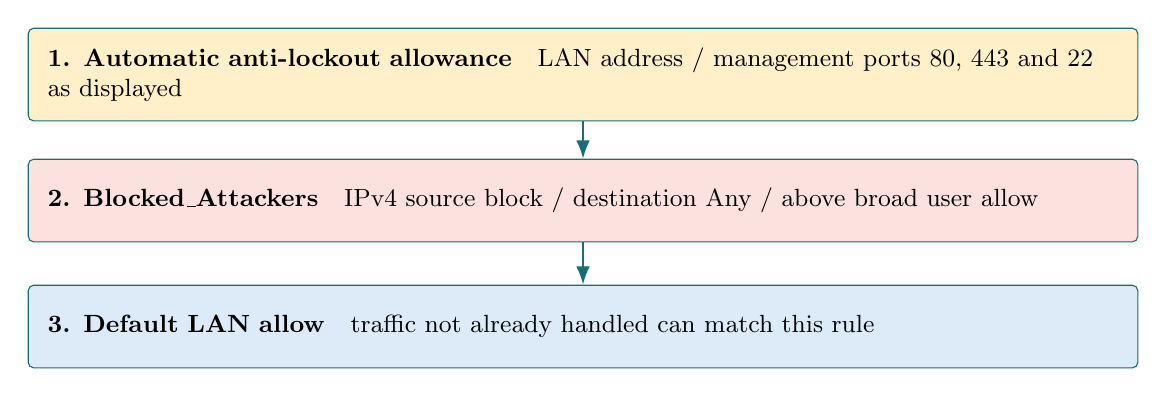
\begin{tikzpicture}[font=\small,rule/.style={draw=steel,rounded corners=2pt,align=left,text width=13.6cm,minimum height=1.05cm,inner sep=7pt}]
\node[rule,fill=goldpale] (auto) at (0,0) {\textbf{1. Automatic anti-lockout allowance}\quad LAN address / management ports 80, 443 and 22 as displayed};
\node[rule,fill=redteamlight] (deny) at (0,-1.6) {\textbf{2. Blocked\_Attackers}\quad IPv4 source block / destination Any / above broad user allow};
\node[rule,fill=blueteamlight] (allow) at (0,-3.2) {\textbf{3. Default LAN allow}\quad traffic not already handled can match this rule};
\draw[-{Latex},thick,steel] (auto) -- (deny);
\draw[-{Latex},thick,steel] (deny) -- (allow);
\end{tikzpicture}
\captionof{figure}{Observed pfSense rule-order explanation based on \ev{E003}. The automatic management exception remains above the source block. This diagram does not imply that unshown floating or group rules were audited.}
\end{center}

\textbf{Important caveats.} The rule editor's \textbf{Log} checkbox is unchecked in \ev{E001}; this image therefore cannot support a claim that matching block events were recorded in the firewall log. The anti-lockout rule still appears above the block in \ev{E003}. Netgate documents that this automatic allowance overrides ordinary LAN restrictions for administration. It cannot be treated as a complete web-portal denial test.
\screenshot{E001}
\begin{troublebox}[Difficulty Encountered - Proving the Firewall Block]
\textbf{Problem.} A rule in the GUI did not, by itself, prove that the intended requests were denied. The editor also shows logging unchecked, and the final rule list retains anti-lockout above the source block. \textbf{Why.} Management exceptions, existing states and traffic that bypasses the gateway can produce different outcomes. \textbf{Response.} We checked the gateway's ICMP traffic with \texttt{tcpdump} rather than relying on the rule screenshot alone. \textbf{Outcome.} We obtained scoped evidence of a response change. Complete portal denial, endpoint containment and a logged block trail were not established and remain follow-up tests.
\end{troublebox}

\subsection{Verify the Specific Path That Was Tested}
We chose \texttt{tcpdump} on pfSense to compare packets on the actual gateway interface. Filtering on ICMP and Bruno's address kept the verification focused on one path and made the request/reply behaviour easier to compare before and after the rule change.
\begin{cmdbox}[Observed on pfSense - shell, not the Kali sensor]
\begin{reportcode}
tcpdump -ni em1 icmp and host 192.168.50.100
\end{reportcode}
\end{cmdbox}
We used \texttt{-n} to keep addresses numeric and \texttt{-i em1} to select the pfSense LAN interface shown in the record. The capture showed request/reply pairs around 17:39:24--25, followed by requests without visible replies around 17:40:17--27. That gave us evidence consistent with a change in gateway ICMP handling. It did not answer whether every TCP service or direct peer-to-peer path was blocked, so those became separate verification requirements.

\reportfigure{E003}{Complete gateway ICMP capture and pfSense rule-context screenshot, \ev{E003}.}{Together with the rule reload and visible block counter, the before/after pattern is consistent with gateway ICMP containment. A capture on ingress may still show a packet that the firewall drops, so seeing a request after blocking is not evidence that the block failed.}

\begin{tabularx}{\linewidth}{@{}L{3.4cm}L{3.4cm}X@{}}
\toprule
\textbf{Path / control} & \textbf{Supplied result} & \textbf{Conclusion}\\
\midrule
.100 to .1 / ICMP & Earlier replies; later requests without visible replies & Scoped containment evidence, consistent with the rule change.\\
.100 to .1 / HTTP or HTTPS & No corresponding denial retest supplied & Not established; anti-lockout remains a relevant exception.\\
.100 to .20 or .40 & Direct same-subnet paths available by design & Gateway rule alone cannot establish endpoint containment.\\
Existing TCP sessions & No host-specific state-clearing capture & Existing permitted states may remain relevant until expired or deliberately cleared.\\
Firewall event logging & Editor checkbox unchecked & Matching block-log evidence requires explicit logging and a new test.\\
\bottomrule
\end{tabularx}

\subsection{Recommended Completion of the Containment Test}
Our next defensive priority would be to close the verification gaps exposed by that test. We would enable the relevant rule logging, check fresh connection behaviour and preserve Blue Team management access while testing each intended path separately. The actions below are a \textbf{future verification plan}, not additional steps claimed to have succeeded. We would first back up the configuration and retain local console access so a management-rule error could be recovered safely.
\begin{enumerate}
\item Verify the actual members of \texttt{Blocked\_Attackers}; keep approved management clients separate from test sources. Enable logging on the relevant block rule, save and apply.
\item If the goal includes denying access \emph{to} pfSense's GUI, first create and test a narrow trusted-management allow rule. Only then consider disabling the automatic anti-lockout rule under \textbf{System > Advanced > Admin Access}. Do not remove the only available management path.
\item Inspect \textbf{Diagnostics > States}, filter on \texttt{192.168.50.100}, and remove only the test host's states when an immediate fresh-connection retest is required. Avoid flushing unrelated connections.
\item Run a small, agreed set of fresh ICMP and HTTP/HTTPS checks from Bruno, then repeat the permitted management check from Blue. Verify the target is otherwise healthy so a service outage is not mistaken for a firewall block.
\item Correlate \textbf{Status > System Logs > Firewall}, the specific rule/tracker, and packet observations. Preserve the configured rule, source/destination/protocol and timestamps in the evidence.
\item For traffic between same-subnet endpoints, use a verified host-firewall rule or redesign the lab into routed security zones. Do not claim that adding a gateway alias alone protects that path. Restore the approved test policy after the exercise.
\end{enumerate}

\begin{cmdbox}[pfSense read-only verification commands - after confirming interface names]
\begin{reportcode}
pfctl -sr
pfctl -ss
pfctl -t Blocked_Attackers -T show
tcpdump -ni em1 'host 192.168.50.100 and (icmp or tcp)'
\end{reportcode}
\end{cmdbox}
For that retest, we would use \texttt{pfctl -sr} to inspect loaded rules, \texttt{pfctl -ss} to inspect states, and the table query to check the active block-list contents. These answer different questions from simply viewing the saved GUI fields. The named table must exist; changing it with \texttt{pfctl -T add} would affect runtime state rather than the persistent GUI alias and may be lost on reload. We would run these checks on pfSense, not on the separate Suricata guest.

\subsection{Packet Capture and Endpoint Corroboration}
We also used Wireshark to examine a known exchange between Amina's scanner and Bruno's workstation. The \texttt{ip.addr==192.168.50.100} display filter reduced the view to packets involving the Red source, and the decoded echo reply showed that the two lab hosts could communicate. This helped us corroborate their addresses and the captured path; it did not give us evidence of the FTP exploit or universal sensor coverage.
\screenshot{E050}
\textbf{Follow the same exchange in the later capture view.} The request and reply directions corroborate the scanner and attacker addresses.
\screenshot{E067}
\textbf{Retain the identity-bearing view.} This additional supplied screenshot records the same exchange with the student's overlay, not a new set of attacks.
\screenshot{E068}

\begin{cmdbox}[Recommended Kali capture and offline inspection]
\begin{reportcode}
ip -brief address
sudo tshark -D
sudo tshark -i eth0 -f 'net 192.168.50.0/24' -a duration:60 \
  -w capture.pcapng
tshark -r capture.pcapng \
  -Y 'ip.addr==192.168.50.100 && (http.request || icmp)'
\end{reportcode}
\end{cmdbox}
Replace \texttt{eth0} only after checking the actual sensor interface. The \texttt{-f} expression is a capture filter; \texttt{-Y} is a Wireshark display filter. The 60-second limit bounds this verification capture. HTTPS application payloads are not exposed just by adding an HTTP filter. Review traffic visibility before assuming that a quiet capture means the target received no attack.

Fahdil supplied the workstation-side view by opening VulnBank from Windows 10 and recording the application state. This gave us another vantage point on the lab, but it was not a Windows Security log investigation. To complete that part in a repeat exercise, we would first verify local audit policy, then inspect the relevant logon and process events on the system that generated them. A packet blocked before authentication need not create a failed-logon event.
\screenshot{E018}
\textbf{Later workstation observation.} The following image preserves the subsequent application view without claiming that the unchanged screen proves an absence of attacks.
\screenshot{E019}
\begin{cmdbox}[Recommended on PC2 Windows PowerShell - recent security events]
\begin{reportcode}
Get-WinEvent -FilterHashtable @{
  LogName = 'Security'
  Id = 4624,4625,4688
  StartTime = (Get-Date).AddHours(-2)
} -MaxEvents 100 | Select-Object TimeCreated, Id, Message
\end{reportcode}
\end{cmdbox}
On the Ubuntu application host, inspect the \emph{configured} Apache access/error log paths and application service logs. A normal HTTP access log often omits POST bodies, so it cannot be promised to contain every literal login payload. \texttt{who} and shell history likewise do not reliably record an unregistered backdoor shell. No missing log is reconstructed as fabricated evidence here.

Looking back, our defensive chain was a configuration check, a working live alert view, identification of the exercise source, a source-based gateway rule and a focused packet comparison. Amina's scanner difficulties and the missing endpoint/raw-log evidence showed us where our visibility was incomplete. Those limits shaped our next recommendations: repair scanner readiness, enable scoped firewall logging, verify endpoint controls, and repeat the same permitted and denied paths before claiming closure.

\subsection{Joint Exercise Timeline}
\begin{tabularx}{\linewidth}{@{}L{3.4cm}X L{2.4cm}@{}}
\toprule
\textbf{Displayed time} & \textbf{Event and decision relevance} & \textbf{Evidence}\\
\midrule
11:04 EDT & Nmap discovers eight lab addresses; establish the asset map. & E030\\
11:44 EDT & Full TCP scan begins for the two selected targets. & E033\\
16:23:08, offset absent & Suricata records Nmap User-Agent events to gateway HTTP. & E006/E007\\
12:33:28 -0400 & FTP backdoor shell opens with root on .40. & E039/E040\\
13:07:39, guest login record & SSH last-login message identifies .100 as source; a later screenshot shows a separate session. & E047\\
17:39--17:40, pfSense clock & ICMP response pattern changes after the block-rule configuration. & E003\\
13:41:22, Kali display & Hydra candidate line and HTTP401 errors; manual verification needed. & E042\\
17:47:35 UTC & Simulated 5000 FCFA transfer receipt. & E045\\
12:59:58 / 13:26:53 EDT & SCAP directory growth, but scanner remains incomplete. & E079/E080\\
\bottomrule
\end{tabularx}
This table preserves source-local timestamps and follows the narrative rather than claiming a fully synchronized event order. The subset does not support a defensible mean time to detect, mean time to respond, total attack count or network-wide block rate.

\partheading{06 / FINDINGS}{Vulnerability Findings and Risk Assessment}
\label{sec:findings}
\subsection{Rating Method and Scope of Conclusions}
The register combines demonstrated exploitation, service-policy exposures and defensive-control observations. It does not represent eight OpenVAS results. Each issue is counted once, even when several screenshots show it; a password change and SSH verification are consequences of F01 rather than additional independent root vulnerabilities.

For prioritization, likelihood and impact are each rated 1--5: 1 is limited/unlikely, 3 is material/possible, and 5 is severe/highly likely within the assessed configuration. The product determines the report's qualitative band: Low 1--5, Medium 6--11, High 12--19, Critical 20--25. These are \textbf{analyst risk judgments for a production analogue}, not measured probabilities or exam marks. Findings deliberately introduced into a training target remain serious if carried into a real environment.

Only F01 is assigned a published CVSS value here: NVD lists CVE-2011-2523 as \textbf{CVSS v3.1 9.8 Critical}, with vector \texttt{CVSS:3.1/AV:N/AC:L/PR:N/UI:N/S:U/C:H/I:H/A:H}. The complete vector and source are retained. Other ratings are qualitative; the available context does not justify attaching fabricated scanner scores. CVSS is owned by FIRST and used with attribution under its published terms.

\small
\begin{longtable}{@{}L{0.8cm}L{4.4cm}L{2.7cm}L{1.7cm}L{1.2cm}L{4.4cm}@{}}
\toprule
\textbf{ID} & \textbf{Finding} & \textbf{Asset} & \textbf{Rating} & \textbf{L x I} & \textbf{Evidence / state}\\
\midrule\endhead
F01 & Backdoored FTP provides root & 192.168.50.40 & Critical & 5 x 5 & E039/E040; demonstrated; open.\\
F02 & Anonymous writable SMB share & 192.168.50.40 & High & 4 x 4 & E035/E036; policy observed; open.\\
F03 & Anonymous FTP authentication & 192.168.50.40 & Medium & 3 x 3 & E032/E036; policy observed; open.\\
F04 & Advertised default VulnBank administrator credential & 192.168.50.20 & High & 4 x 4 & E041--E045, D4; corroborated; open.\\
F05 & Cleartext web application listeners & 192.168.50.20 & Medium & 3 x 3 & E031/E034; observed; open.\\
F06 & pfSense default-password warning & 192.168.50.1 & High & 3 x 5 & E002/E003; observed; open.\\
F07 & Flat subnet limits gateway containment & Lab /24 & Medium & 3 x 3 & Architecture and E003; partial containment only.\\
F08 & Block-rule logging disabled & 192.168.50.1 & Medium & 3 x 2 & E001/E003; retest pending.\\
\bottomrule
\end{longtable}
\normalsize

\begin{center}
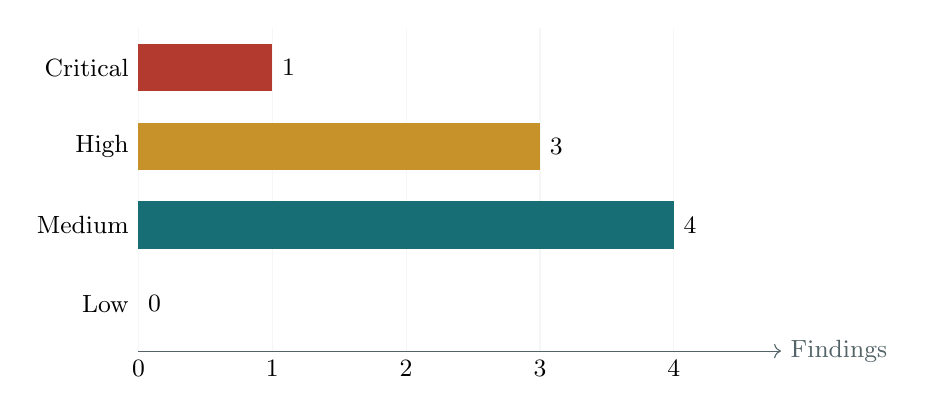
\begin{tikzpicture}[font=\small,x=1.7cm,y=1cm]
\draw[->,muted] (0,0) -- (4.8,0) node[right]{Findings};
\foreach \tick in {0,1,2,3,4} {
  \draw[lightgrey] (\tick,0) -- (\tick,4.1);
  \node[below] at (\tick,0) {\tick};
}
\fill[redteam] (0,3.3) rectangle (\CriticalCount,3.9);
\fill[accentgold] (0,2.3) rectangle (\HighCount,2.9);
\fill[steel] (0,1.3) rectangle (\MediumCount,1.9);
\node[left] at (0,3.6) {Critical};
\node[left] at (0,2.6) {High};
\node[left] at (0,1.6) {Medium};
\node[left] at (0,0.6) {Low};
\node[right] at (\CriticalCount,3.6) {\CriticalCount};
\node[right] at (\HighCount,2.6) {\HighCount};
\node[right] at (\MediumCount,1.6) {\MediumCount};
\node[right] at (0,0.6) {\LowCount};
\end{tikzpicture}
\captionof{figure}{Severity distribution of the eight deduplicated report findings. Counts are generated from the findings register, not from a scanner export or screenshot count.}
\end{center}

\subsection{F01 - Backdoored FTP Provides Root Access}
\label{finding:F01}
\textbf{Asset / evidence:} \texttt{192.168.50.40}; \ev{E032}, \ev{E038}--\ev{E040}, \ev{E046}, \ev{E047}; Red Team PDF, physical pages 7--10. \textbf{Severity: Critical. Status: Open.}

The target exposes vsftpd 2.3.4 and a successful session to the backdoor listener on TCP6200. The resulting shell is root and identifies the correct host. This is materially stronger than a version-only match to CVE-2011-2523. The demonstrated account modification corroborates high integrity impact; root privileges also imply serious confidentiality and availability potential. No destructive outage was attempted.

\textbf{Business impact.} In the SecureTech scenario, equivalent access could expose application files and credentials, permit unauthorized account changes and disrupt services. These are consequences of the demonstrated capability, not claims that real customer data was stolen.

\textbf{Remediation / owner.} Rayan, as target owner, should remove the affected image from any non-test network and rebuild from trusted supported media. Replace the backdoored service rather than merely changing FTP authentication policy; rotate credentials exposed to the compromised host and verify account integrity. Preserve a deliberately vulnerable snapshot only in an isolated teaching environment.

\textbf{Closure test.} On the rebuilt authorized target, verify approved service versions, confirm the backdoor listener is absent, ensure no unauthorized account changes remain and repeat the bounded initial-access check under approval. No completed rebuild/retest is supplied.

\subsection{F02 - Anonymous Writable SMB Share}
\textbf{Asset / evidence:} \texttt{192.168.50.40}; \ev{E035}, \ev{E036}. \textbf{Severity: High. Status: Open.}

The SMB enumeration result classifies the \texttt{tmp} share as anonymous \texttt{READ/WRITE}. An unauthenticated party could potentially access or alter files exposed by that share. The screenshot records the access policy; it does not establish what valuable files existed, a successful file upload, or execution of a file placed there.

\textbf{Remediation / owner.} Rayan should remove unintended guest access, require named accounts, restrict share permissions and filesystem ACLs, and allow SMB only between required systems. Test that guest/null-session access is denied while a permitted test account still performs its approved operation. Record both outcomes before closure.

\subsection{F03 - Anonymous FTP Authentication}
\textbf{Asset / evidence:} \texttt{192.168.50.40}; \ev{E032}, \ev{E036}. \textbf{Severity: Medium. Status: Open.}

The FTP check returns \texttt{Anonymous FTP login allowed (FTP code 230)}. Unauthenticated access is established; sensitive content, upload permissions and actual data loss are not. This finding is distinct from F01: a trusted service can still have an unsafe anonymous-access policy, and a backdoored binary remains unsafe even after anonymous login is disabled.

\textbf{Remediation / owner.} Remove unnecessary FTP or replace it with an approved authenticated transfer service. Restrict any required download-only area to intended public content and narrow its network reach. Verify anonymous authentication fails and authorized access still works. Rayan owns the service configuration, with Blue Team verification.

\subsection{F04 - Advertised Default VulnBank Administrator Credential}
\textbf{Asset / evidence:} \texttt{192.168.50.20}; \ev{E017}, \ev{E028}, \ev{E041}--\ev{E045}; Red Team PDF, physical pages 11--14. \textbf{Severity: High. Status: Open.}

The public login page advertises \texttt{admin/admin}. Hydra reports the same candidate but also emits repeated errors. The operator report records a successful manual login, and the following screenshots demonstrate administrator access and a simulated payment. The combined record corroborates the default-credential path without requiring the error-laden automation to be treated as reliable proof by itself.

\textbf{Business impact.} Equivalent defaults in production could allow an unauthorized party to use privileged functions and alter accounts or transactions. The 5,000 FCFA receipt is an illustration of demo impact only.

\textbf{Remediation / owner.} The application owner should remove seeded credentials and public hints from non-lab deployments, require unique secrets and privileged-account protection, enforce server-side authorization for every sensitive operation, and monitor authentication failures. Rayan maintains the application; Fahdil can provide Blue Team verification. A clean invalid/valid login comparison and role check are needed before assessing lockout or rate-limiting behaviour.

\subsection{F05 - Cleartext Web Application Listeners}
\textbf{Asset / evidence:} \texttt{192.168.50.20}, TCP80 and TCP3000; \ev{E031}, \ev{E034}, \ev{E041}, \ev{E043}. \textbf{Severity: Medium. Status: Open.}

The application is served over HTTP, and the displayed HTTPS connection attempt is refused. Both Apache and the direct Express listener expose the application. This establishes lack of observed transport protection on those paths, not a successful interception of a password. The risks include disclosure or modification of credentials and session data to a party able to observe or alter the transport path.

\textbf{Remediation / owner.} Configure HTTPS with a verified certificate at the approved entry point, redirect or disable unneeded HTTP routes, set appropriate secure session-cookie attributes, and bind or filter the direct application listener so it cannot unintentionally bypass the entry-point controls. Test browser/login behaviour on both listeners; do not rely only on a changed header or a different page length.

\subsection{F06 - pfSense Default Administrator Password Warning}
\textbf{Asset / evidence:} \texttt{192.168.50.1}; \ev{E002}, \ev{E003}. \textbf{Severity: High. Status: Open.}

The management interface explicitly warns that the current password is set to its default value. In a shared lab, that weakens the security of the device controlling routing and firewall policy. The capture demonstrates the warning, not an attacker login to pfSense or a successful unauthorized rule change.

\textbf{Remediation / owner.} Marshall should change the administrator secret, use named administrative accounts and appropriate authentication controls, restrict management to trusted clients or a separate management network, and retain a verified recovery method. Retest that the default credential is rejected while approved administration remains available. A completed password change is not present in the supplied record.

\subsection{F07 - Flat Subnet Limits Gateway Containment}
\textbf{Asset / evidence:} \texttt{192.168.50.0/24}; the bridged topology, \ev{E003}, \ev{E005}, \ev{E023}, \ev{E025}--\ev{E027}, \ev{E030}. \textbf{Severity: Medium. Status: Partially contained.}

The gateway rule produced scoped ICMP containment evidence, but the hosts share a connected subnet. Direct layer-2 traffic can avoid pfSense, and several configuration stages show secondary NAT adapters. The management anti-lockout rule also remains in place. This is an architectural/control-coverage limitation, not a new exploit demonstrated against every host.

\textbf{Remediation / owner.} Marshall and the target owners should review active routes/uplinks, use host firewalls for required immediate endpoint restrictions, and design separate routed target, attacker and management zones if network-level segmentation is required. Provide an explicit mirror/TAP or validated capture arrangement for the passive sensor. Retest gateway-bound, routed and same-subnet paths separately; each has a different enforcement point.

\subsection{F08 - Block-Rule Logging Disabled in the Captured Configuration}
\textbf{Asset / evidence:} \texttt{192.168.50.1}; \ev{E001}, \ev{E003}. \textbf{Severity: Medium. Status: Retest pending.}

The visible rule editor has packet logging unchecked. The configuration and packet excerpt support a containment observation, but not a matching firewall-event trail for that rule. Without the relevant events, the team cannot reliably explain which rule acted on each rejected connection or reconstruct a complete block timeline.

\textbf{Remediation / owner.} Marshall should enable logging for the relevant security rules, configure retention/time synchronization, protect log access and perform a small new test that produces a matching source/destination/protocol/tracker record. Logging every benign packet is not required and can overwhelm a constrained VM. Existing-state handling and legitimate Blue access must be checked alongside the logging change.

\subsection{Additional Observations Not Counted as Confirmed Findings}
\begin{itemize}
\item \textbf{Plaintext application passwords:} the UI warns of intentional exposure and the Red Team PDF reports it, but the supplied screenshot shows a column heading rather than visible password values. Confirm storage and API behaviour before assigning a separate demonstrated finding.
\item \textbf{Other legacy services and distccd:} identified as leads or described in the source report, but not separately exploited or fully validated here. Do not assign a CVE from a banner alone.
\item \textbf{OpenVAS readiness:} an assessment/tooling blocker, not a vulnerability discovered on the target network. It remains an action item and a coverage limitation.
\item \textbf{Windows policy, lateral movement and persistence:} the record does not establish their successful exploitation or completed hardening. Analysis is clearly separated from evidence of execution.
\end{itemize}

\subsection{Threat Model and Scenario Impact}
\begin{tabularx}{\linewidth}{@{}L{2.7cm}L{3.4cm}X@{}}
\toprule
\textbf{Critical asset} & \textbf{Threat / entry vector} & \textbf{Consequence and control focus}\\
\midrule
Server accounts and files & Untrusted internal host reaches backdoored FTP or open shares & Account takeover and file tampering; trusted rebuild, access policy and segmented reachability.\\
Application balances and sessions & Default administrator secret or cleartext login path & Privileged misuse and session exposure; remove defaults, HTTPS and server-side authorization.\\
Firewall administration & Shared default credential and broad management access & Policy manipulation or loss of network control; protected administration and audited changes.\\
Employee workstation & Possible access from a compromised peer & Potential downstream exposure, not demonstrated compromise; host firewall, supported OS and log collection.\\
Detection evidence & Gaps in capture visibility, parsing and rule logging & Incomplete incident reconstruction; validated capture paths, preserved originals and scoped security logging.\\
Assessment coverage & Scanner feed/import failure & Unknown undiscovered weaknesses; repair readiness and repeat the authorized scan before claiming completeness.\\
\bottomrule
\end{tabularx}

\begin{center}
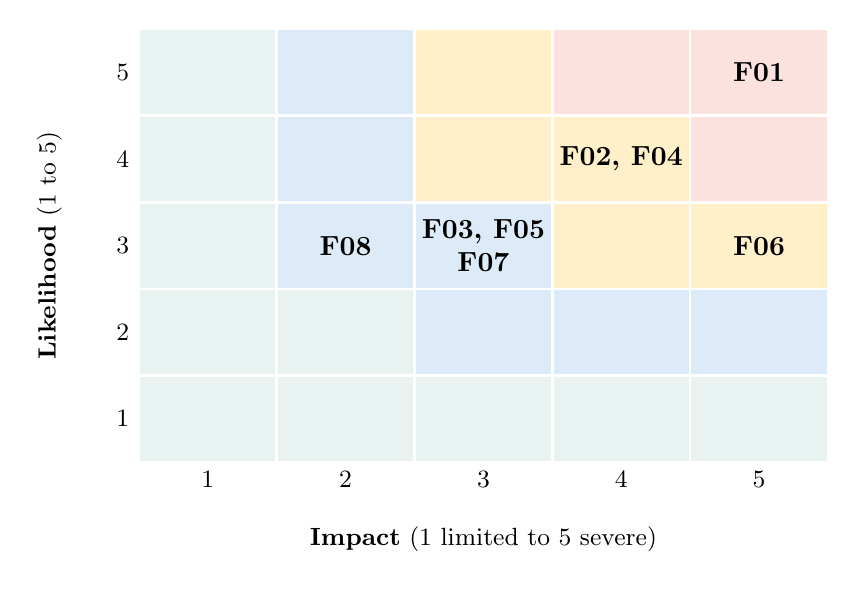
\begin{tikzpicture}[x=1.75cm,y=1.1cm,font=\small]
\foreach \likelihood in {1,...,5} {
  \foreach \impact in {1,...,5} {
    \pgfmathtruncatemacro{\risk}{\likelihood*\impact}
    \ifnum\risk>19 \def\shade{redteamlight}\else
      \ifnum\risk>11 \def\shade{goldpale}\else
        \ifnum\risk>5 \def\shade{blueteamlight}\else \def\shade{pale}\fi
      \fi
    \fi
    \filldraw[fill=\shade,draw=white,line width=1pt] (\impact-1,\likelihood-1) rectangle (\impact,\likelihood);
  }
  \node[left] at (0,\likelihood-0.5) {\likelihood};
  \node[below] at (\likelihood-0.5,0) {\likelihood};
}
\node[font=\bfseries] at (4.5,4.5) {F01};
\node[font=\bfseries] at (3.5,3.5) {F02, F04};
\node[font=\bfseries] at (4.5,2.5) {F06};
\node[align=center,font=\bfseries] at (2.5,2.5) {F03, F05\\F07};
\node[font=\bfseries] at (1.5,2.5) {F08};
\node[below=7mm] at (2.5,0) {\textbf{Impact} (1 limited to 5 severe)};
\node[rotate=90] at (-0.65,2.5) {\textbf{Likelihood} (1 to 5)};
\end{tikzpicture}
\captionof{figure}{Analyst risk matrix for the eight registered findings. Colour is supplemented by IDs; empty cells are not evidence of tested-safe assets.}
\end{center}

\partheading{07 / RESPONSE PLAN}{Hardening, Recovery and Retesting}
\label{sec:hardening}
\subsection{Prioritized Remediation Register}
The following priorities are proposed for the lab and its production analogue, not recorded completion dates. \textbf{P0} means before the next hostile exercise; \textbf{P1} means before the next assessed baseline. Physical asset ownership does not change team membership: Rayan assists target recovery as owner, while Blue Team validates the defensive result.

\small
\begin{longtable}{@{}L{1.3cm}L{4.5cm}L{2.8cm}L{7.0cm}@{}}
\toprule
\textbf{Priority} & \textbf{Action} & \textbf{Owner} & \textbf{Acceptance / evidence required}\\
\midrule\endhead
P0 & Isolate and rebuild affected FTP target (F01) & Rayan; Blue validates & Approved image/service; no6200 backdoor; required service tests pass; lab-account restoration recorded.\\
P0 & Replace default app and firewall credentials (F04/F06) & Application owner; Marshall & Default login rejected; unique approved account succeeds; management access preserved.\\
P1 & Restrict anonymous SMB/FTP (F02/F03) & Rayan & Anonymous access denied; least-privilege test account retains only required access.\\
P1 & Require HTTPS and review direct3000 access (F05) & Application owner & Correct certificate and login/session behaviour; direct listener not an unintended control bypass.\\
P1 & Validate enforcement paths (F07) & Marshall and all owners & Fresh tests for gateway, inter-zone and same-subnet paths; unintended secondary uplinks removed or controlled.\\
P1 & Enable scoped logging and preserve timestamps (F08) & Marshall; Fahdil & Matching event with rule/tracker and endpoints; retention configured; clocks recorded.\\
P1 & Repair OpenVAS readiness & Amina & Valid feed owner, imported port list and scan config, connected scanner, completed authorized scan/export.\\
P1 & Establish Windows defensive baseline & Fahdil & Supported/maintained OS, effective firewall profiles, account policy and enabled event collection recorded.\\
\bottomrule
\end{longtable}
\normalsize

\subsection{Verification Commands and Their Limits}
Run follow-up checks on the appropriate machine after an approved change. They are included for reproducibility, not as evidence that remediation occurred during the original exercise.
\begin{cmdbox}[Ubuntu application host - patch and service verification]
\begin{reportcode}
sudo apt update
apt list --upgradable
sudo apt upgrade
dpkg-query -W apache2 openssh-server
sudo apache2ctl configtest
sudo systemctl status apache2 --no-pager
sudo ss -lntp
\end{reportcode}
\end{cmdbox}
Use the supported Ubuntu application guest, not the intentionally obsolete Metasploitable image, for routine patch-management demonstrations. Record package versions and vendor security status; a backported fix may retain the same upstream banner, so a banner change is not a required or sufficient proof of patching. Review the proposed transaction before confirming an upgrade and validate application functionality afterward.

\begin{cmdbox}[PC2 Windows PowerShell - record the defensive baseline]
\begin{reportcode}
Get-ComputerInfo | Select-Object WindowsProductName, WindowsVersion
Get-HotFix | Sort-Object InstalledOn -Descending | Select-Object -First 10
Get-NetFirewallProfile | Select-Object Name, Enabled
net accounts
\end{reportcode}
\end{cmdbox}
An update list is useful inventory, not proof that all vulnerabilities are patched. Document the actual support/extended-update status of Windows 10. Do not claim MFA, lockout or audit policies were enforced merely because a report recommends them.

For Linux host-level containment, first identify the active firewall framework, established connections and management allow rules. Enabling UFW without that review can lock out administrators or interfere with Docker and other rules. An explicit incoming rule on a target can protect that \emph{target}; it does not turn the passive Suricata guest into a network-wide firewall. The report therefore favors a controlled, verifiable policy change over an unqualified copy-paste block command.

\subsection{Incident Response Workflow}
\begin{enumerate}
\item \textbf{Detect and record.} Capture the alert's time, signature, direction and affected service. Preserve the relevant source log and original evidence hash.
\item \textbf{Triage.} Confirm scope and attribution; compare Bruno's test source with Amina's approved scanner and exclude unrelated background traffic. Determine whether there is evidence of access, not just a signature hit.
\item \textbf{Contain.} Apply the narrowest control that acts on the actual path. In the documented case this was a pfSense source block; same-subnet endpoints require separate controls. Preserve management access and evidence.
\item \textbf{Eradicate.} Remove the underlying backdoored software/default credentials or unsafe policy. A temporary IP block alone does not remediate the vulnerable target.
\item \textbf{Recover.} Restore known-good lab images/accounts, validate required services and permitted Blue access, then lift temporary rules only under the agreed test policy.
\item \textbf{Learn and close.} Compare the same before/after tests, attach rule and log evidence, record residual gaps and assign ownership. Keep the issue open where the retest is absent.
\end{enumerate}

\subsection{Red and Blue Team Handoffs}
\begin{center}
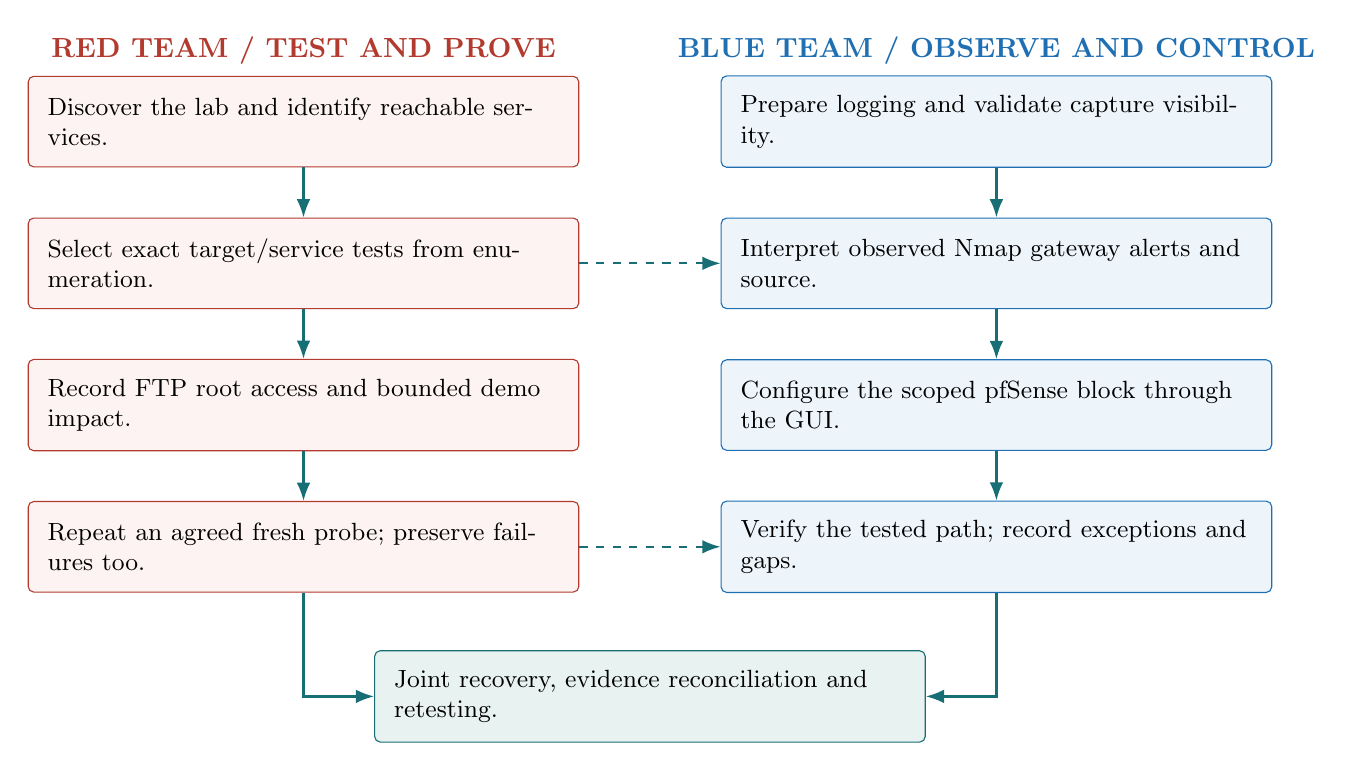
\begin{tikzpicture}[font=\small,task/.style={text width=6.5cm,align=left,minimum height=1.15cm,inner sep=7pt,rounded corners=2pt},link/.style={-{Latex},thick,steel}]
\node[text=redteam,font=\bfseries] at (0,0.9) {RED TEAM / TEST AND PROVE};
\node[text=blueteam,font=\bfseries] at (8.8,0.9) {BLUE TEAM / OBSERVE AND CONTROL};
\node[task,fill=redteamlight!40,draw=redteam] (r1) at (0,0) {Discover the lab and identify reachable services.};
\node[task,fill=blueteamlight!50,draw=blueteam] (b1) at (8.8,0) {Prepare logging and validate capture visibility.};
\node[task,fill=redteamlight!40,draw=redteam] (r2) at (0,-1.8) {Select exact target/service tests from enumeration.};
\node[task,fill=blueteamlight!50,draw=blueteam] (b2) at (8.8,-1.8) {Interpret observed Nmap gateway alerts and source.};
\node[task,fill=redteamlight!40,draw=redteam] (r3) at (0,-3.6) {Record FTP root access and bounded demo impact.};
\node[task,fill=blueteamlight!50,draw=blueteam] (b3) at (8.8,-3.6) {Configure the scoped pfSense block through the GUI.};
\node[task,fill=redteamlight!40,draw=redteam] (r4) at (0,-5.4) {Repeat an agreed fresh probe; preserve failures too.};
\node[task,fill=blueteamlight!50,draw=blueteam] (b4) at (8.8,-5.4) {Verify the tested path; record exceptions and gaps.};
\node[task,fill=pale,draw=steel] (joint) at (4.4,-7.3) {Joint recovery, evidence reconciliation and retesting.};
\draw[link] (r1) -- (r2);\draw[link] (r2) -- (r3);\draw[link] (r3) -- (r4);
\draw[link] (b1) -- (b2);\draw[link] (b2) -- (b3);\draw[link] (b3) -- (b4);
\draw[link,dashed] (r2) -- (b2);
\draw[link,dashed] (r4) -- (b4);
\draw[link] (r4.south) |- (joint.west);
\draw[link] (b4.south) |- (joint.east);
\end{tikzpicture}
\captionof{figure}{Operational strategy and handoffs. Dashed links indicate evidence correlation or an agreed verification handoff, not proof that every offensive action has a matching defender log.}
\end{center}

\subsection{Minimum Retest Record}
For each change, record the finding ID, responsible operator, baseline service state, source/destination IP, protocol/port, command or GUI action, exact time/offset, observed result, corresponding log/rule entry and recovery action. A valid closure requires both the unwanted path to fail and the approved path to continue working. No supplied screenshot demonstrates closure of F01--F06; F07 has scoped containment evidence and F08 awaits logged retesting.

\partheading{08 / CONCLUSIONS}{Outcomes, Coverage and Lessons Learned}
\subsection{Assessment Conclusion}
The strongest technical result is verified root access to Metasploitable2 through the FTP backdoor, followed by bounded account-control effects. The application evidence corroborates a default-credential concern and administrator capabilities in a deliberately insecure banking simulation. The successful Blue Team observation was detection of the Red source's gateway reconnaissance, followed by a source-block configuration and a gateway ICMP response change.

The main residual risks are the unrepaired target weaknesses, broad trust within the flat bridged segment, exposed administrative defaults, incomplete logging proof and the blocked automated assessment. These are actionable results even though the exercise did not complete every expected demonstration. Professional reporting preserves that distinction instead of presenting the preparatory guides' expected outcomes as measured facts.

\subsection{Examination Task Coverage}
\small
\begin{longtable}{@{}L{0.7cm}L{3.5cm}L{1.1cm}L{10.1cm}@{}}
\toprule
\textbf{Task} & \textbf{Requirement} & \textbf{Marks} & \textbf{Evidence-backed coverage and remaining gap}\\
\midrule\endhead
1 & Lab design and documentation & 5 & Setup, full-IP topology and eight-address inventory included. Some installation screens/resources remain reconstructed or reported.\\
2 & Reconnaissance and discovery & 4 & Eight hosts in E030; asset inventory and interpretation included.\\
3 & Service enumeration & 4 & Service/version, HTTP, SMB and FTP checks in E031--E036. UDP and all application routes not comprehensively tested.\\
4 & Threat modelling and risk & 4 & Asset-threat model, ranked risk register and matrix included as analysis.\\
5 & Vulnerability assessment & 6 & Manual findings documented; automated OpenVAS work incomplete. No scan export or fabricated five-result scanner table.\\
6 & Controlled initial access & 6 & FTP root access, exact target and identity checks in E037--E040.\\
7 & Web assessment & 6 & Rejected SQLi, default-credential path and simulated impact. Authentication and transport concerns identified; two independently successful OWASP exploit demonstrations are not established.\\
8 & Credential assessment & 4 & Default credential exposure and corroborated application access; historical Hydra error retained. No completed hash-cracking or Windows policy audit supplied.\\
9 & Escalation / persistence analysis & 5 & Initial session already root; account manipulation documented. No separate escalation or deployed persistence falsely claimed.\\
10 & Post-exploitation / lateral analysis & 5 & Account modification and SSH to the same target evidenced; no successful cross-host pivot shown.\\
11 & Traffic and log investigation & 5 & Suricata alerts/stats, Wireshark ICMP and pfSense capture interpreted. Full raw logs/PCAP absent.\\
12 & Hardening and response & 5 & GUI block configured, scoped observation, detailed response and retest plan. Broader controls remain recommendations.\\
13 & Professional reporting & 11 & This report includes scope, methodology, findings, evidence, impact, risk, recommendations, conclusions and source register.\\
\midrule
 & \textbf{Total available} & \textbf{70} & Marks are reproduced from the examination brief; no grade is claimed.\\
\bottomrule
\end{longtable}
\normalsize

\subsection{Lessons for the Next Exercise}
\begin{itemize}
\item Validate the network path, not just the IP address: a gateway is not automatically an inter-host enforcement point.
\item Make scanner readiness a pre-exercise gate. Installation and an accessible login page are not sufficient.
\item Use targeted manual checks to guide controlled exploitation when automated assessment is blocked, without pretending that coverage is equivalent.
\item Preserve failed attempts, original commands, offsets and evidence hashes. Corrected commands must not overwrite the historical record.
\item Test copied PDF command characters. The earlier hyphen substitution was a real operational failure despite visually correct pages.
\item Collect the required continuous videos and raw logs/PCAPs. A screenshot set and a new report cannot replace missing primary artifacts.
\end{itemize}

\subsection{Deliverable Completeness}
This PDF contains the professional report, architecture diagram, asset inventory, manual findings, risk register, hardening/response plan and all supplied unique screenshots. Exact duplicates are indexed. The build sources and hash inventories accompany it. The examination also requires one identity-bearing video per task and source artifacts where applicable; no such videos or raw scan/capture exports were provided, and they have not been manufactured.

\partheading{09 / REFERENCES}{Source Documents and Technical References}
\label{sec:sources}
\subsection{Supplied PDFs}
Page references below use \textbf{physical PDF page numbers}, including any cover page. Seven files were read/extracted, representing five unique documents and 70 unique pages. The two pairs of guide PDFs are byte-identical and have not been counted twice as independent evidence. Source PDFs remain unchanged even where this report corrects their interpretation.

\begin{description}[leftmargin=1cm,style=nextline]
\item[D1]\phantomsection\label{src:D1}\textbf{Ethical Hacking SETTING A SUMMER 2026.pdf}, 5 pages. Examination scenario, authorized lab scope, required infrastructure/deliverables, 13 tasks and 70-mark allocation. Pages3--4 provide the task requirements. The required DVWA/Juice Shop example differs from the team's confirmed VulnBank implementation and is disclosed as a lab deviation.
\item[D2]\phantomsection\label{src:D2}\textbf{CYS4151\_Lab\_Network\_Configuration.pdf}, 20 pages; identical copy \textbf{lab-network-configuration.pdf}. Preparatory build/addressing guide. Expected resource allocations, DVWA deployment and universal routing/visibility claims are not treated as actual execution evidence.
\item[D3]\phantomsection\label{src:D3}\textbf{CYS4151\_Post-Configuration\_Execution\_Guide.pdf}, 20 pages; identical copy \textbf{post-configuration-execution-guide.pdf}. Planned commands and outcomes. This report corrects the unsupported escalation, scan, pivot, parsing and containment claims where actual evidence differs.
\item[D4]\phantomsection\label{src:D4}\textbf{RED TEAM REPORT.pdf}, 15 pages. Operators: Bruno and Rayan. Pages3--6 discovery/enumeration; pages7--10 FTP access and account-control demonstration; pages11--14 web testing and simulated transfer. The overlapping text on page15 is not counted as additional evidence; the preceding narrative and original screenshots support the analysis. The reported manual login is identified as operator testimony corroborated by the captured session.
\item[D5]\phantomsection\label{src:D5}\textbf{amina openvas.pdf}, 10 pages. Amina's incomplete Task5 assessment. Pages2--3 scope/resources; pages4--7 feed and target-creation evidence; pages7--9 diagnosis/limitations/remediation; page10 evidence inventory. Reported resource increases and five attempts are preserved without adopting unproven causal claims or the obsolete rebuild command as a validated remedy.
\end{description}

\subsection{Public Technical References}
\begin{enumerate}
\item NIST, \emph{Technical Guide to Information Security Testing and Assessment}, SP800-115. \referenceurl{https://doi.org/10.6028/NIST.SP.800-115}
\item OWASP, \emph{Web Security Testing Guide}. \referenceurl{https://owasp.org/www-project-web-security-testing-guide/}
\item NVD, \emph{CVE-2011-2523: vsftpd backdoor}, including CVSS v3.1 score and vector. Consulted 05 October 2026. \referenceurl{https://nvd.nist.gov/vuln/detail/CVE-2011-2523}
\item FIRST, \emph{Common Vulnerability Scoring System v3.1: Specification Document}. CVSS is owned by FIRST and used by permission under the published terms. \referenceurl{https://www.first.org/cvss/v3.1/specification-document}
\item Netgate, \emph{Rule Methodology}: inbound filtering, states and automatic anti-lockout rules. \referenceurl{https://docs.netgate.com/pfsense/en/latest/firewall/rule-methodology.html}
\item Netgate, \emph{Admin Access}: safely restricting GUI/SSH access before disabling anti-lockout. \referenceurl{https://docs.netgate.com/pfsense/en/latest/config/advanced-admin.html}
\item Netgate, \emph{Viewing Firewall States in the GUI}: filtering and removing host-specific states. \referenceurl{https://docs.netgate.com/pfsense/en/latest/monitoring/status/firewall-states-gui.html}
\item Nmap, \emph{Reference Guide and NSE documentation}. \referenceurl{https://nmap.org/book/man.html}
\item Suricata, \emph{User Guide: output and EVE JSON}. \referenceurl{https://docs.suricata.io/en/latest/output/eve/index.html}
\item Greenbone, \emph{Community Documentation}. Match instructions to installed distribution/package versions. \referenceurl{https://greenbone.github.io/docs/latest/}
\end{enumerate}

\subsection{Build and Verification Record}
This report is built locally with XeLaTeX. The retained \texttt{ActualText} setting protects ASCII command characters in PDF copying. The exact four EVE \texttt{jq} filters in this report were tested with a checksum-verified official jq1.8.1 binary against synthetic valid alerts, a statistics record and a malformed line. That is offline syntax/behaviour validation, \emph{not} replay of the team's unavailable EVE file. No new lab attacks, firewall changes or vulnerability scans were performed in preparing the report.

\appendix
\partheading{SOURCE INDEX}{Source Image Register}
\label{sec:evidence-index}
Every supplied screenshot is listed below, including the ten exact duplicate copies in Rayan's second folder. E081--E090 map to E020--E029 respectively. Each unique image appears in full beside its matching explanation in the main report; the links below return to that figure. There is no separate end-of-document screenshot gallery. The hash prefixes are for readable lookup; the full SHA-256 hashes, original dimensions and paths are in the accompanying image inventory CSV.

\small
\begin{longtable}{@{}L{1.1cm}L{1.1cm}L{8.0cm}L{1.5cm}L{3.6cm}@{}}
\toprule ID & Task & Original source file & Figure & SHA-256 prefix \\ \midrule\endhead
E001 & 12 & ethical hacking screen short/pc 1/blocked attacker ip.png & \ev{E001} & \texttt{F9ACD9198790} \\
E002 & 12 & ethical hacking screen short/pc 1/blocking pc bruno ip on pfsense.png & \ev{E002} & \texttt{FFBA3281334D} \\
E003 & 11/12 & ethical hacking screen short/pc 1/blocking red team.png & \ev{E003} & \texttt{CB8143C32ECD} \\
E004 & 1 & ethical hacking screen short/pc 1/configuring pfsense 2 adapters one NAt.png & \ev{E004} & \texttt{E8190D53A3D3} \\
E005 & 1 & ethical hacking screen short/pc 1/pfsense adapter config bridge.png & \ev{E005} & \texttt{A5FA4A979B2B} \\
E006 & 11 & ethical hacking screen short/pc 1/suricata fast logs 2 .png & \ev{E006} & \texttt{DBA5D79D8D4F} \\
E007 & 11 & ethical hacking screen short/pc 1/suricata fast logs displaying attacker .100 nmap .png & \ev{E007} & \texttt{824074ACCDD2} \\
E008 & 1 & ethical hacking screen short/pc 1/suricata inst1.png & \ev{E008} & \texttt{3BC5ECA78B30} \\
E009 & 1/11 & ethical hacking screen short/pc 1/suricata inst2.png & \ev{E009} & \texttt{7B25587D2129} \\
E010 & 11 & ethical hacking screen short/pc 1/suricata logs.png & \ev{E010} & \texttt{8B582940FEDD} \\
E011 & 11 & ethical hacking screen short/pc 1/suricata stats logs.png & \ev{E011} & \texttt{CE93AE5FD22D} \\
E012 & 1 & ethical hacking screen short/pc 2/Capture d'écran 2026-10-03 144246.png & \ev{E012} & \texttt{8556E96DE388} \\
E013 & 1 & ethical hacking screen short/pc 2/Capture d'écran 2026-10-03 145336.png & \ev{E013} & \texttt{9587B6D1D716} \\
E014 & 1 & ethical hacking screen short/pc 2/Capture d'écran 2026-10-03 145349.png & \ev{E014} & \texttt{0532CBD78F6C} \\
E015 & 1 & ethical hacking screen short/pc 2/Capture d'écran 2026-10-03 150533.png & \ev{E015} & \texttt{E5936327AC33} \\
E016 & 1 & ethical hacking screen short/pc 2/Capture d'écran 2026-10-03 150758.png & \ev{E016} & \texttt{62CC83C843DC} \\
E017 & 1/8 & ethical hacking screen short/pc 2/Capture d'écran 2026-10-03 153545.png & \ev{E017} & \texttt{7EC65439D0F8} \\
E018 & 1/11 & ethical hacking screen short/pc 2/Capture d'écran 2026-10-03 174340.png & \ev{E018} & \texttt{9C143679322E} \\
E019 & 11 & ethical hacking screen short/pc 2/Capture d'écran 2026-10-03 182240.png & \ev{E019} & \texttt{B0F5FCBD65BD} \\
E020 & 1 & ethical hacking screen short/pc 3/allow-vuln.png & \ev{E020} & \texttt{D579A008BBB6} \\
E021 & 1/10 & ethical hacking screen short/pc 3/hacked-meta.png & \ev{E021} & \texttt{DAA51E060F65} \\
E022 & 1 & ethical hacking screen short/pc 3/netcofig-ubuntu1.png & \ev{E022} & \texttt{9C36DAA1C1DD} \\
E023 & 1 & ethical hacking screen short/pc 3/netcofig-ubuntu2.png & \ev{E023} & \texttt{BEE14686AFE8} \\
E024 & 1 & ethical hacking screen short/pc 3/netconfig-metasploitable.png & \ev{E024} & \texttt{345DB817EE65} \\
E025 & 1 & ethical hacking screen short/pc 3/vbox-metasploitable.png & \ev{E025} & \texttt{65CCDB77C244} \\
E026 & 1 & ethical hacking screen short/pc 3/vbox-ubuntu1.png & \ev{E026} & \texttt{517628B3F69C} \\
E027 & 1 & ethical hacking screen short/pc 3/vbox-ubuntu2.png & \ev{E027} & \texttt{BEFA4D3CB87D} \\
E028 & 1 & ethical hacking screen short/pc 3/vul-bank.png & \ev{E028} & \texttt{903FC9B0B6AF} \\
E029 & 1/3 & ethical hacking screen short/pc 3/vul-status.png & \ev{E029} & \texttt{6DFD887250DB} \\
E030 & 2 & ethical hacking screen short/pc 4/T1-S1.png & \ev{E030} & \texttt{64A7B4D43E27} \\
E031 & 2/3 & ethical hacking screen short/pc 4/T1-S2(1).png & \ev{E031} & \texttt{67ADF703E8E3} \\
E032 & 3 & ethical hacking screen short/pc 4/T1-S2(2).png & \ev{E032} & \texttt{A0CA0A32D7F5} \\
E033 & 3 & ethical hacking screen short/pc 4/T3-S1.png & \ev{E033} & \texttt{C57CF97A94CE} \\
E034 & 3 & ethical hacking screen short/pc 4/T3-S2.png & \ev{E034} & \texttt{1426029A4B1B} \\
E035 & 3 & ethical hacking screen short/pc 4/T3-S3(1).png & \ev{E035} & \texttt{8FBAC6D2B906} \\
E036 & 3/5 & ethical hacking screen short/pc 4/T3-S3(2).png & \ev{E036} & \texttt{D797638C7939} \\
E037 & 6 & ethical hacking screen short/pc 4/T6-S1.png & \ev{E037} & \texttt{352D6639FF10} \\
E038 & 6 & ethical hacking screen short/pc 4/T6-S2.png & \ev{E038} & \texttt{766E97A5CABB} \\
E039 & 6 & ethical hacking screen short/pc 4/T6-S3.png & \ev{E039} & \texttt{C21CB7A042C7} \\
E040 & 6/9 & ethical hacking screen short/pc 4/T6-S4.png & \ev{E040} & \texttt{A06367499871} \\
E041 & 7 & ethical hacking screen short/pc 4/T7-S1.png & \ev{E041} & \texttt{A68CF856D29B} \\
E042 & 8 & ethical hacking screen short/pc 4/T7-S2.png & \ev{E042} & \texttt{5C62398D0777} \\
E043 & 7/8 & ethical hacking screen short/pc 4/T7-S3.png & \ev{E043} & \texttt{E08BB711FAA8} \\
E044 & 7 & ethical hacking screen short/pc 4/T7-S4.png & \ev{E044} & \texttt{39AE4F408D69} \\
E045 & 7 & ethical hacking screen short/pc 4/T7-S5.png & \ev{E045} & \texttt{C8E61F322BE1} \\
E046 & 9/10 & ethical hacking screen short/pc 4/T9-S1.png & \ev{E046} & \texttt{B9629B8B5C1F} \\
E047 & 10 & ethical hacking screen short/pc 4/T9-S2.png & \ev{E047} & \texttt{1DC82AED9A70} \\
E048 & 1 & ethical hacking screen short/pc 5/screen1.png & \ev{E048} & \texttt{514B8C66C86F} \\
E049 & 5 & ethical hacking screen short/pc 5/screen2.png & \ev{E049} & \texttt{0534B81C1851} \\
E050 & 2/11 & ethical hacking screen short/pc 5/screen3.png & \ev{E050} & \texttt{4D787DEC9A78} \\
E051 & 5 & ethical hacking screen short/pc 5/SCREEN4.PNG & \ev{E051} & \texttt{0AA1EC8F86D3} \\
E052 & 5 & ethical hacking screen short/pc 5/screen5.png & \ev{E052} & \texttt{88CE3B2BA66C} \\
E053 & 5 & ethical hacking screen short/pc 5/screen6.png & \ev{E053} & \texttt{C45BB5DCDB5E} \\
E054 & 1 & ethical hacking screen short/pc 5/Screenshot 2026-10-03 143056.png & \ev{E054} & \texttt{F6A976C597D4} \\
E055 & 1 & ethical hacking screen short/pc 5/Screenshot 2026-10-03 143320.png & \ev{E055} & \texttt{CF5D29A39BCC} \\
E056 & 1 & ethical hacking screen short/pc 5/Screenshot 2026-10-03 143718.png & \ev{E056} & \texttt{B7F8EF8C0210} \\
E057 & 1 & ethical hacking screen short/pc 5/Screenshot 2026-10-03 152446.png & \ev{E057} & \texttt{ED539B6CB678} \\
E058 & 5 & ethical hacking screen short/pc 5/Screenshot 2026-10-03 152747.png & \ev{E058} & \texttt{DA35D3743660} \\
E059 & 5 & ethical hacking screen short/pc 5/Screenshot 2026-10-03 153936.png & \ev{E059} & \texttt{7048519D5209} \\
E060 & 5 & ethical hacking screen short/pc 5/Screenshot 2026-10-03 154616.png & \ev{E060} & \texttt{78A18DD25A7D} \\
E061 & 5 & ethical hacking screen short/pc 5/Screenshot 2026-10-03 155514.png & \ev{E061} & \texttt{9BD106917D4E} \\
E062 & 5 & ethical hacking screen short/pc 5/Screenshot 2026-10-03 155614.png & \ev{E062} & \texttt{6608A7B763F7} \\
E063 & 5 & ethical hacking screen short/pc 5/Screenshot 2026-10-03 160436.png & \ev{E063} & \texttt{42E463FDAB57} \\
E064 & 5 & ethical hacking screen short/pc 5/Screenshot 2026-10-03 160458.png & \ev{E064} & \texttt{1F9FA9E50B1C} \\
E065 & 5 & ethical hacking screen short/pc 5/Screenshot 2026-10-03 160524.png & \ev{E065} & \texttt{1C57667A4D29} \\
E066 & 5 & ethical hacking screen short/pc 5/Screenshot 2026-10-03 160925.png & \ev{E066} & \texttt{B5F8C90DC06D} \\
E067 & 11 & ethical hacking screen short/pc 5/Screenshot 2026-10-03 162415.png & \ev{E067} & \texttt{80D4ED70AB03} \\
E068 & 11 & ethical hacking screen short/pc 5/Screenshot 2026-10-03 162450.png & \ev{E068} & \texttt{F4D24579D44B} \\
E069 & 5 & ethical hacking screen short/pc 5/Screenshot 2026-10-03 162749.png & \ev{E069} & \texttt{DF646C683AFF} \\
E070 & 5 & ethical hacking screen short/pc 5/Screenshot 2026-10-03 163708.png & \ev{E070} & \texttt{232A7D4BDABA} \\
E071 & 1 & ethical hacking screen short/pc 5/Screenshot 2026-10-03 165237.png & \ev{E071} & \texttt{6B978E92D06A} \\
E072 & 1 & ethical hacking screen short/pc 5/Screenshot 2026-10-03 165353.png & \ev{E072} & \texttt{EBF942199A89} \\
E073 & 5 & ethical hacking screen short/pc 5/Screenshot 2026-10-03 171010.png & \ev{E073} & \texttt{CC386900199A} \\
E074 & 5 & ethical hacking screen short/pc 5/Screenshot 2026-10-03 171043.png & \ev{E074} & \texttt{C980EC13C455} \\
E075 & 5 & ethical hacking screen short/pc 5/Screenshot 2026-10-03 171827.png & \ev{E075} & \texttt{848BE4004375} \\
E076 & 5 & ethical hacking screen short/pc 5/Screenshot 2026-10-03 173024.png & \ev{E076} & \texttt{880360C9DB2E} \\
E077 & 5 & ethical hacking screen short/pc 5/Screenshot 2026-10-03 173956.png & \ev{E077} & \texttt{8DBFEBDD5A06} \\
E078 & 5 & ethical hacking screen short/pc 5/Screenshot 2026-10-03 175946.png & \ev{E078} & \texttt{04C7CD2F58D7} \\
E079 & 5 & ethical hacking screen short/pc 5/Screenshot 2026-10-03 180015.png & \ev{E079} & \texttt{5315CCF28E64} \\
E080 & 5 & ethical hacking screen short/pc 5/Screenshot 2026-10-03 182702.png & \ev{E080} & \texttt{05DF22AE2732} \\
E081 & 1 & rayan screen shorts/allow-vuln.png & \ev{E020} & \texttt{D579A008BBB6} \\
E082 & 1/10 & rayan screen shorts/hacked-meta.png & \ev{E021} & \texttt{DAA51E060F65} \\
E083 & 1 & rayan screen shorts/netcofig-ubuntu1.png & \ev{E022} & \texttt{9C36DAA1C1DD} \\
E084 & 1 & rayan screen shorts/netcofig-ubuntu2.png & \ev{E023} & \texttt{BEE14686AFE8} \\
E085 & 1 & rayan screen shorts/netconfig-metasploitable.png & \ev{E024} & \texttt{345DB817EE65} \\
E086 & 1 & rayan screen shorts/vbox-metasploitable.png & \ev{E025} & \texttt{65CCDB77C244} \\
E087 & 1 & rayan screen shorts/vbox-ubuntu1.png & \ev{E026} & \texttt{517628B3F69C} \\
E088 & 1 & rayan screen shorts/vbox-ubuntu2.png & \ev{E027} & \texttt{BEFA4D3CB87D} \\
E089 & 1 & rayan screen shorts/vul-bank.png & \ev{E028} & \texttt{903FC9B0B6AF} \\
E090 & 1/3 & rayan screen shorts/vul-status.png & \ev{E029} & \texttt{6DFD887250DB} \\
\bottomrule\end{longtable}\normalsize


\end{document}